\documentclass{beamer}

\mode<presentation> {
\usetheme{Madrid}
}
\usepackage{graphicx}
\usepackage{booktabs} 
\usepackage{wrapfig}

\title[CNNs]{Computer Vision with CNN}

\author{Behnia - Heydari}
\institute[AUT]
{
Amirkabir University of Technology \\ 
\medskip
\textit{}
}
\date{May 21, 2019}

\begin{document}

\begin{frame}
\titlepage
\end{frame}

\begin{frame}
\frametitle{Overview}
\tableofcontents
\end{frame}

\section{Motivation}

\begin{frame}
\frametitle{Cameras Everywhere}
\begin{columns}[c]

\column{.4\textwidth}
\textbf{Smartphones}
\begin{itemize}
\item Exploding number of sensors vs. humans

\end{itemize}
\column{.6\textwidth}

\begin{figure}
	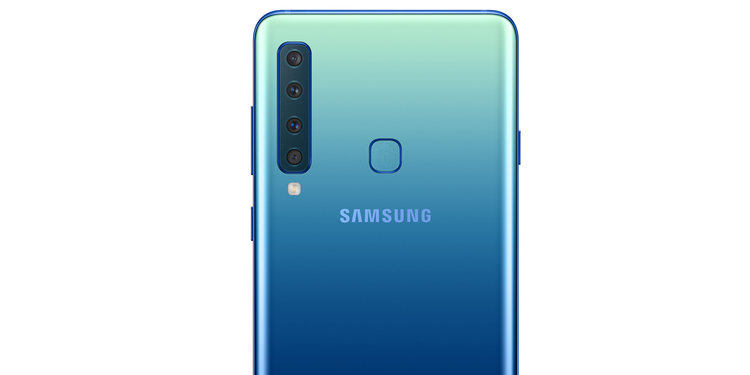
\includegraphics[height=180pt]{Pics/samsung.jpg}
\end{figure}
\end{columns}
\end{frame}

\begin{frame}
\frametitle{ConvNets Everywhere}
\centering
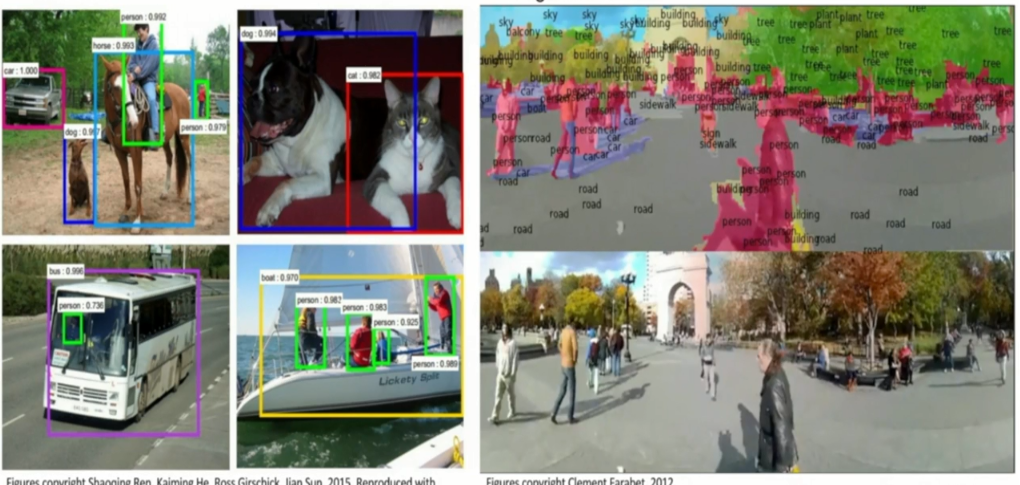
\includegraphics[width=0.9\linewidth]{Pics/ex1.PNG}
\end{frame}
\begin{frame}
\frametitle{ConvNets Everywhere}
\centering
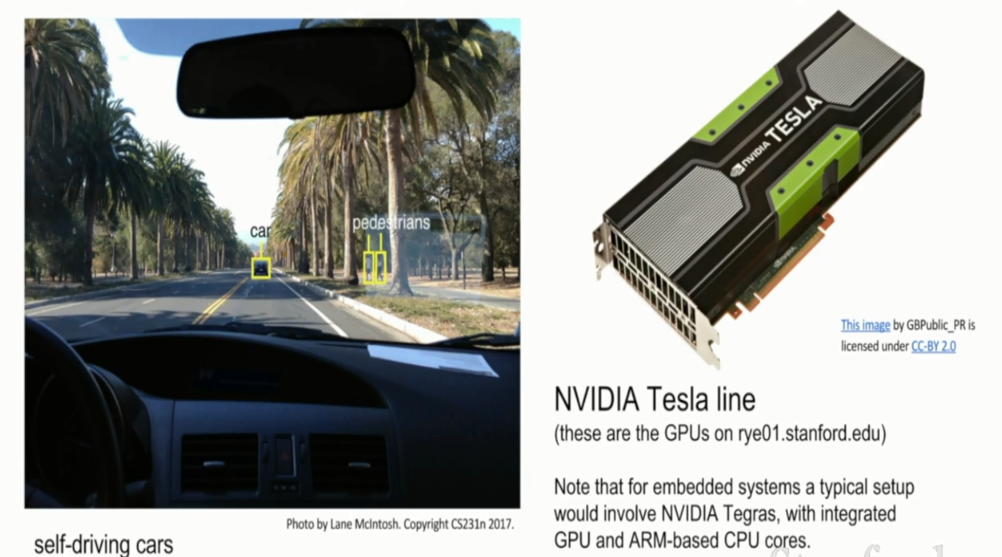
\includegraphics[width=0.9\linewidth]{Pics/ex2.PNG}
\end{frame}
\begin{frame}
\frametitle{ConvNets Everywhere}
\centering
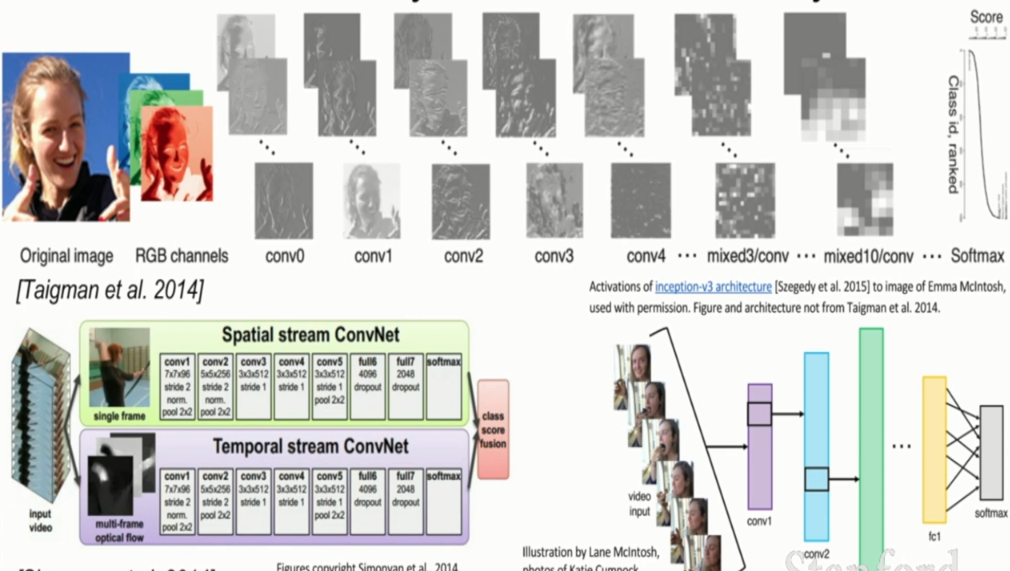
\includegraphics[width=0.9\linewidth]{Pics/ex3.PNG}
\end{frame}
\begin{frame}
\frametitle{ConvNets Everywhere}
\centering
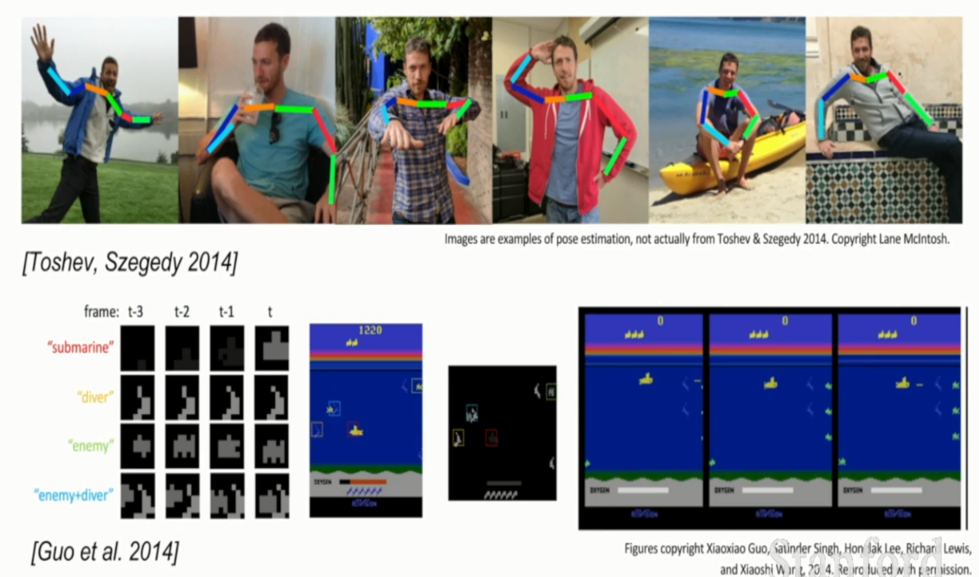
\includegraphics[width=0.9\linewidth]{Pics/ex4.PNG}
\end{frame}
\begin{frame}
\frametitle{ConvNets Everywhere}
\centering
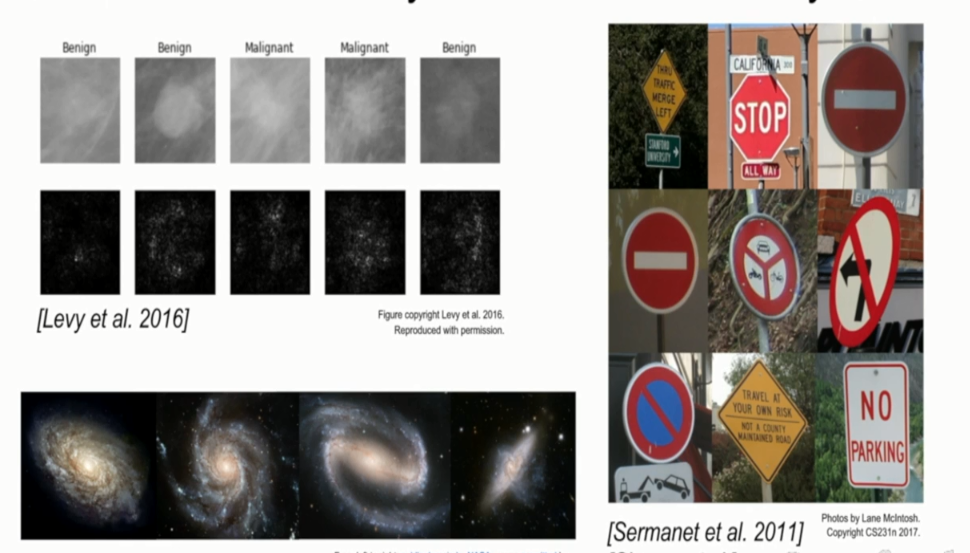
\includegraphics[width=0.9\linewidth]{Pics/ex5.PNG}
\end{frame}


\begin{frame}
	\frametitle{Neat Dataset}
	\begin{figure}
		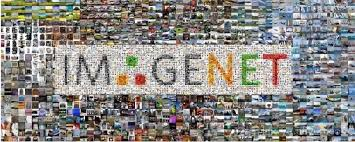
\includegraphics[width=\linewidth]{Pics/image_net.jpeg}
	\end{figure}
\end{frame}

\section{ImageNet Challenge}
\begin{frame}
\frametitle{Role of CNN}
\begin{figure}
	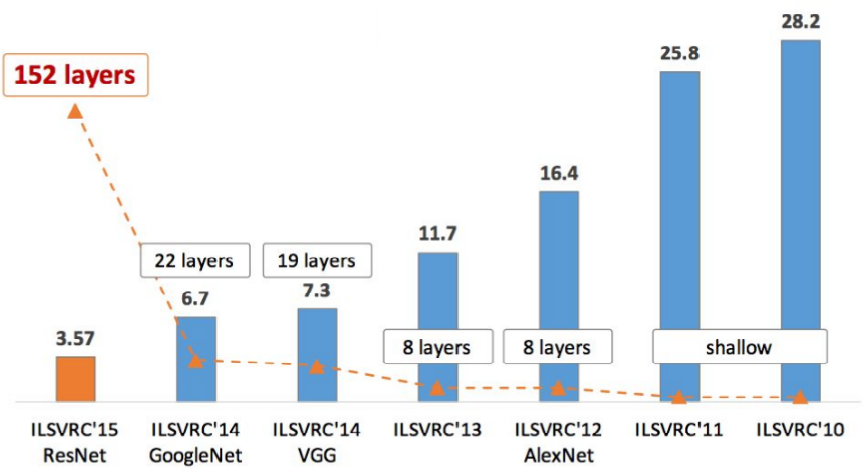
\includegraphics[width=\linewidth]{Pics/imagenet_acc.png}
\end{figure}
\end{frame}

\section{From Cat's Brain to ResNet (Classification)}
\begin{frame}
\frametitle{Cat's Brain}
\begin{columns}[c]
	\column{.4\textwidth}
	\textbf{Types of cells:}
\begin{itemize}
	\item simple cells
	\item complex cells
	\item hypercomplex cells
\end{itemize}
\column{.6\textwidth}

\begin{figure}
	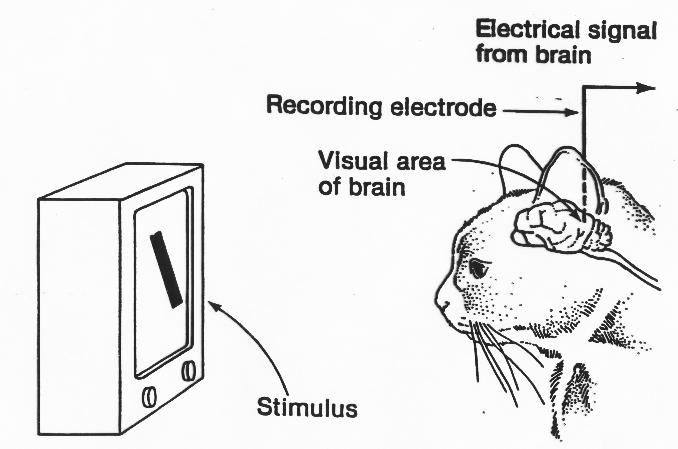
\includegraphics[width=\linewidth]{Pics/cats.jpg}
\end{figure}
\end{columns}
\end{frame}

\begin{frame}
\frametitle{CNN}

	\begin{figure}
		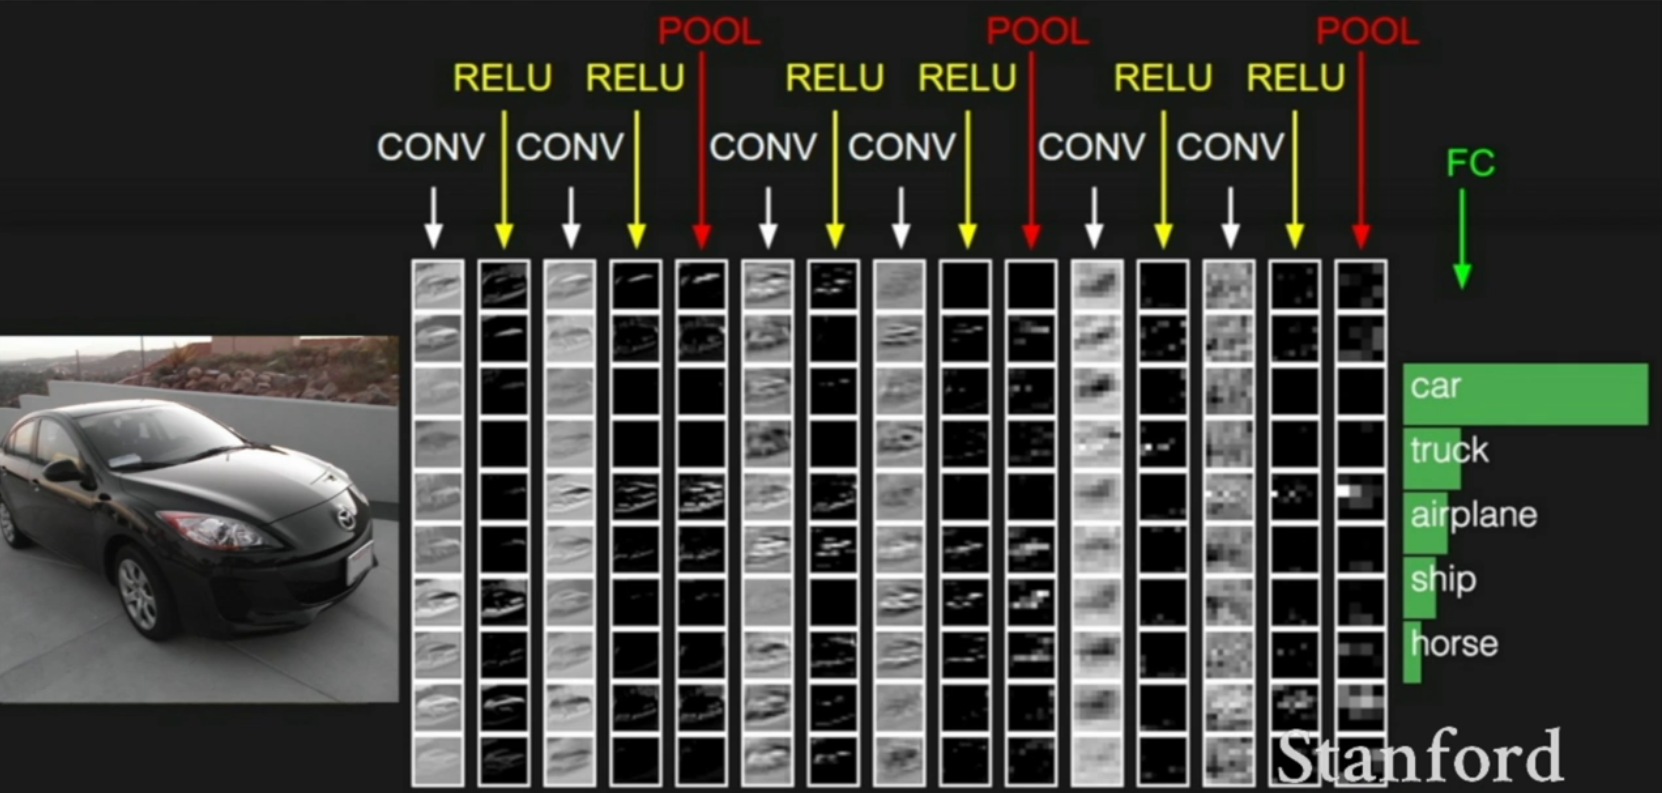
\includegraphics[width=\linewidth]{Pics/cexample.png}
	\end{figure}

\end{frame}
\begin{frame}
\frametitle{Convolution}

\begin{figure}
	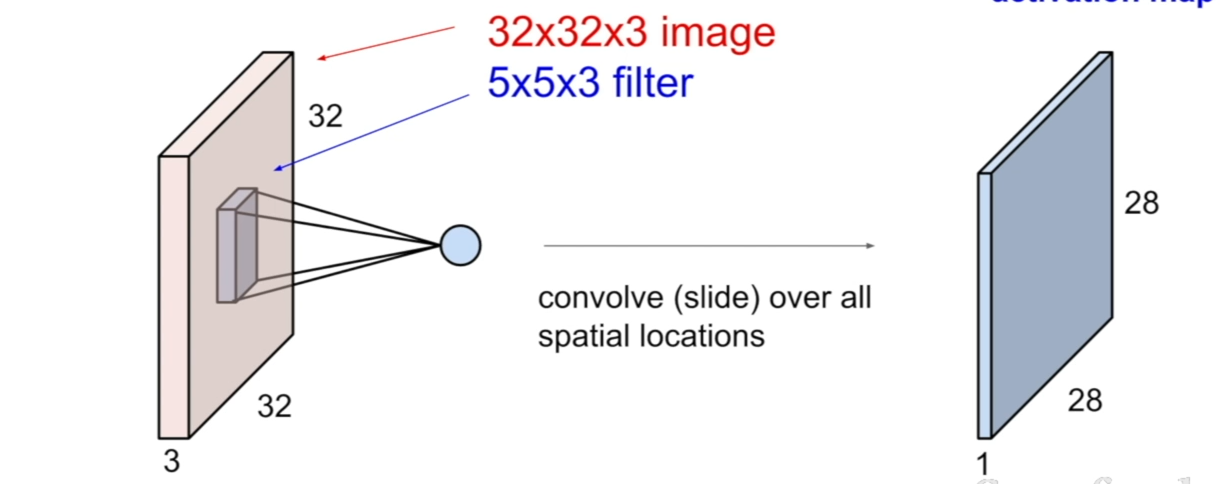
\includegraphics[width=\linewidth]{Pics/cnlayer.png}
	\caption{Convolution Layer}
\end{figure}

\end{frame}

\begin{frame}
\frametitle{Complexity of Features}

\begin{figure}
	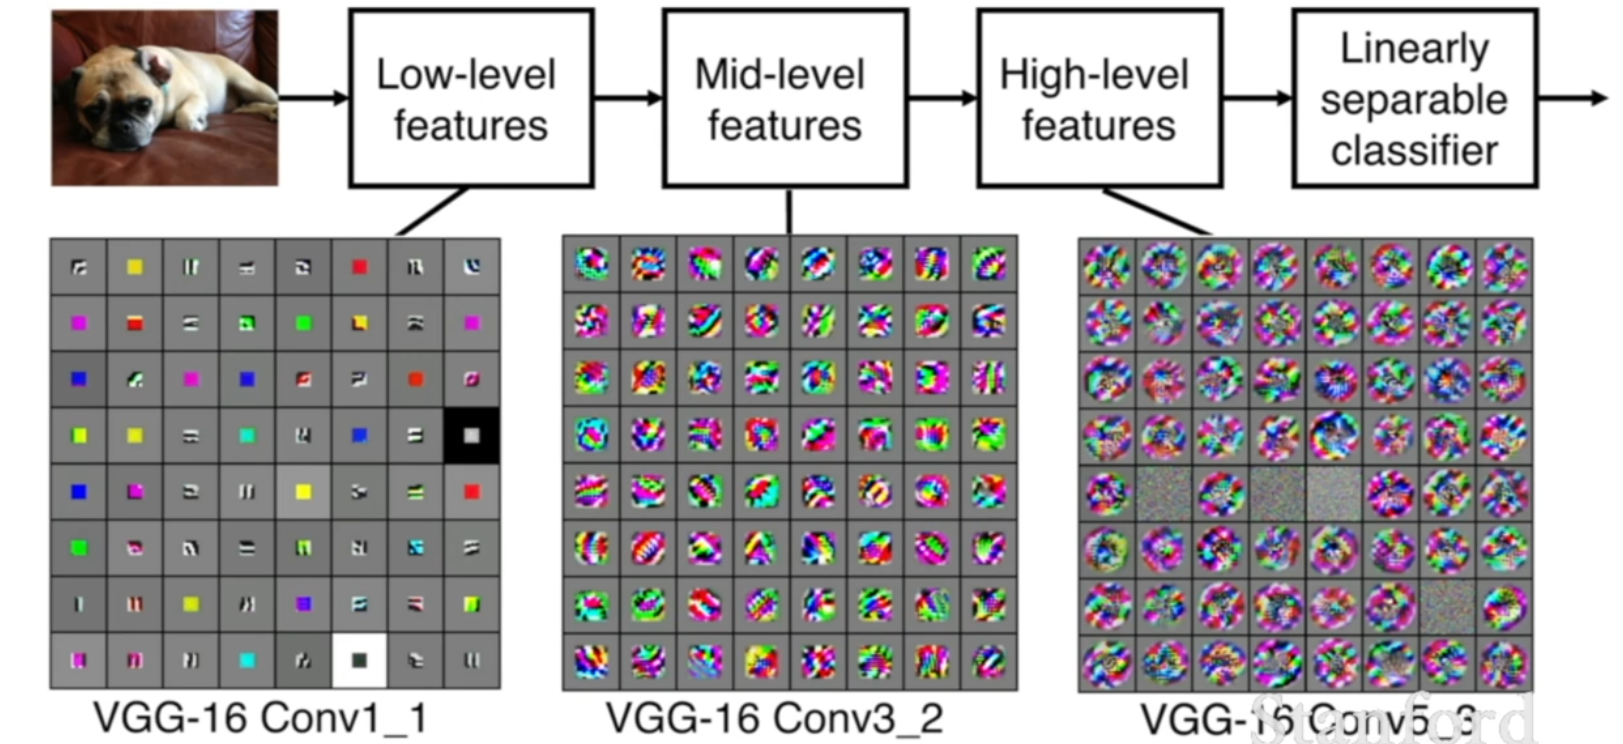
\includegraphics[width=\linewidth]{Pics/hlayer.png}
	\caption{complexity of features in each layer}
\end{figure}
\end{frame}

\begin{frame}
\frametitle{Complexity of Features}

\begin{figure}
	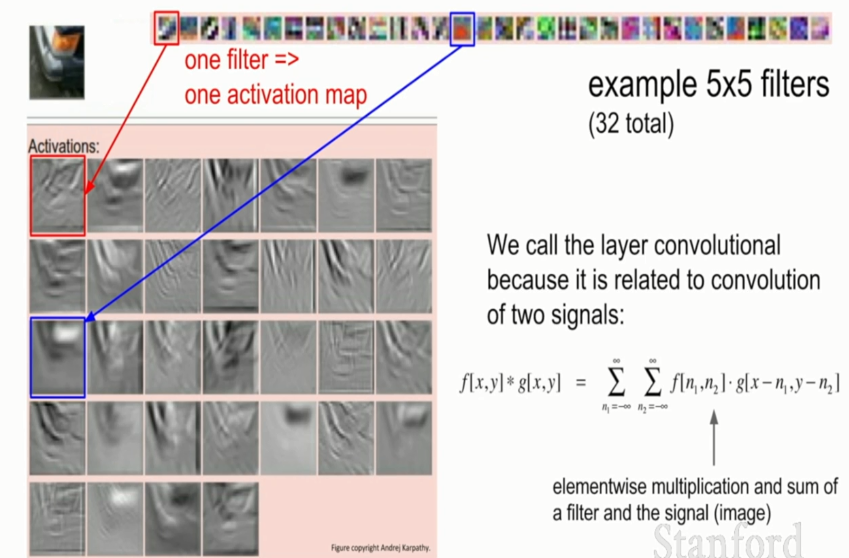
\includegraphics[width=.8\linewidth]{Pics/ex7.PNG}
	\caption{complexity of each layer output}
\end{figure}

\end{frame}

\begin{frame}
\frametitle{Sliding a Filter}
\begin{figure}
	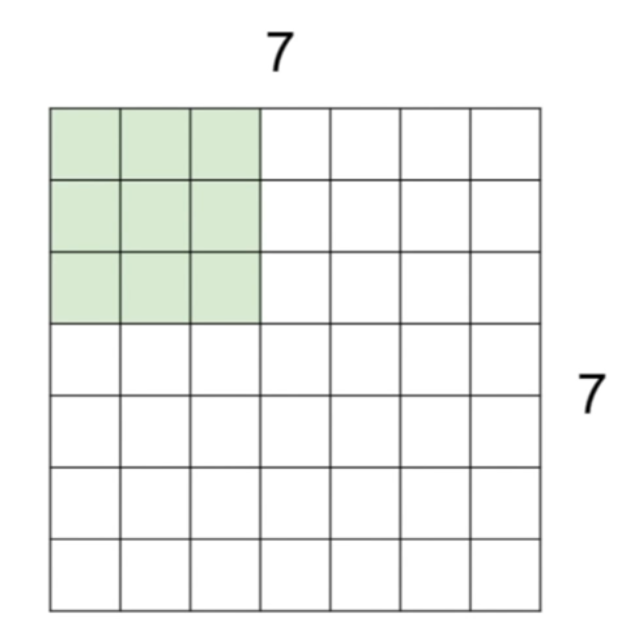
\includegraphics[width=.5\linewidth]{Pics/clook.png}
	\caption{filtering example}
\end{figure}
\end{frame}

\begin{frame}
\frametitle{Sliding a Filter}
\begin{figure}
	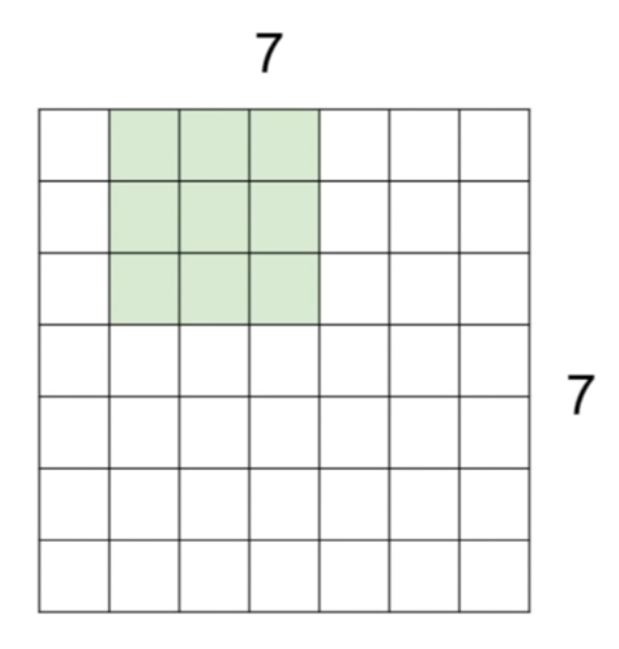
\includegraphics[width=.5\linewidth]{Pics/clook2.png}
	\caption{filtering example}
\end{figure}
\end{frame}

\begin{frame}
\frametitle{Sliding a Filter}
\begin{figure}
	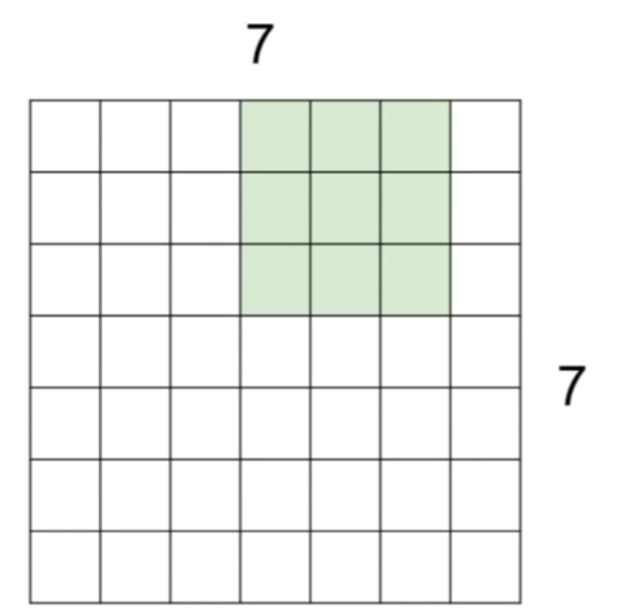
\includegraphics[width=.5\linewidth]{Pics/clook3.png}
	\caption{filtering example}
\end{figure}
\end{frame}

\begin{frame}
\frametitle{Sliding a Filter}
 {\color{red}
 What if using a 3*3 filter with stride 3 ?!
	}
\begin{figure}
	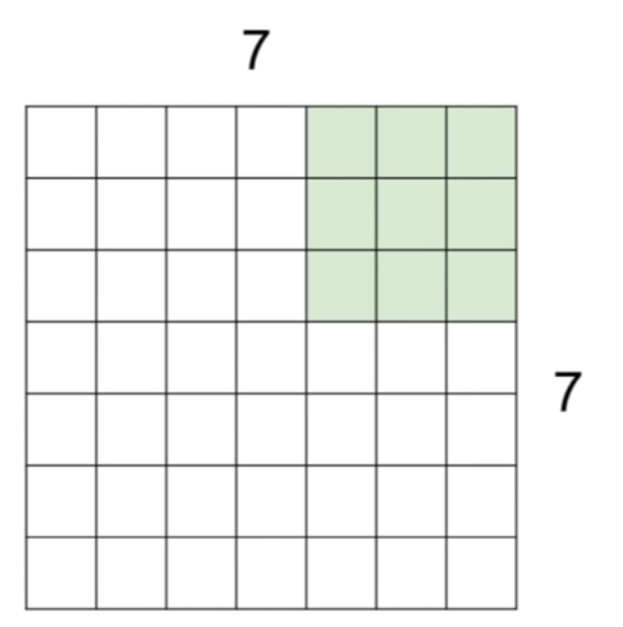
\includegraphics[width=.5\linewidth]{Pics/clook4.png}
	\caption{filtering example}
\end{figure}

\end{frame}

\begin{frame}
\frametitle{Padding}
\begin{figure}
	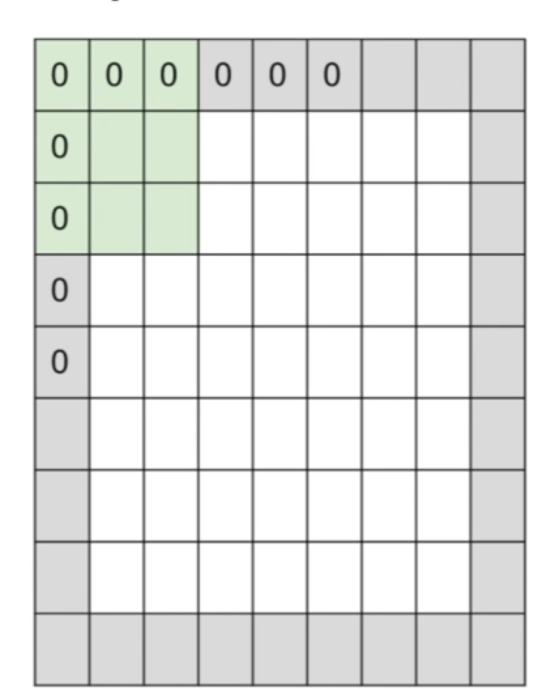
\includegraphics[width=.4\linewidth]{Pics/padding.png}
	\caption{Padding: control output size}
\end{figure}
\end{frame}

\begin{frame}
\frametitle{Summary}
\begin{itemize}
	\item Accept a volume of size N x N 
	\item requires 4 hyper parameters:
	\begin{itemize}
		\item Filter's spatial extent F
		\item Filter's Stride S
		\item Amount of zero padding P
		\item Number of kernels ($\times depth \times$)
	\end{itemize}
	
     \item Produces a volume of size $M \times M$
     \begin{itemize}
     	\item M = $ \frac{(N - F + 2p)}{S} + 1 $
     	\item Number of parameters : $ (F \times F \times D + b) \times k $
     \end{itemize}
\end{itemize}

\end{frame}

\begin{frame}
\frametitle{CNN}

\begin{figure}
	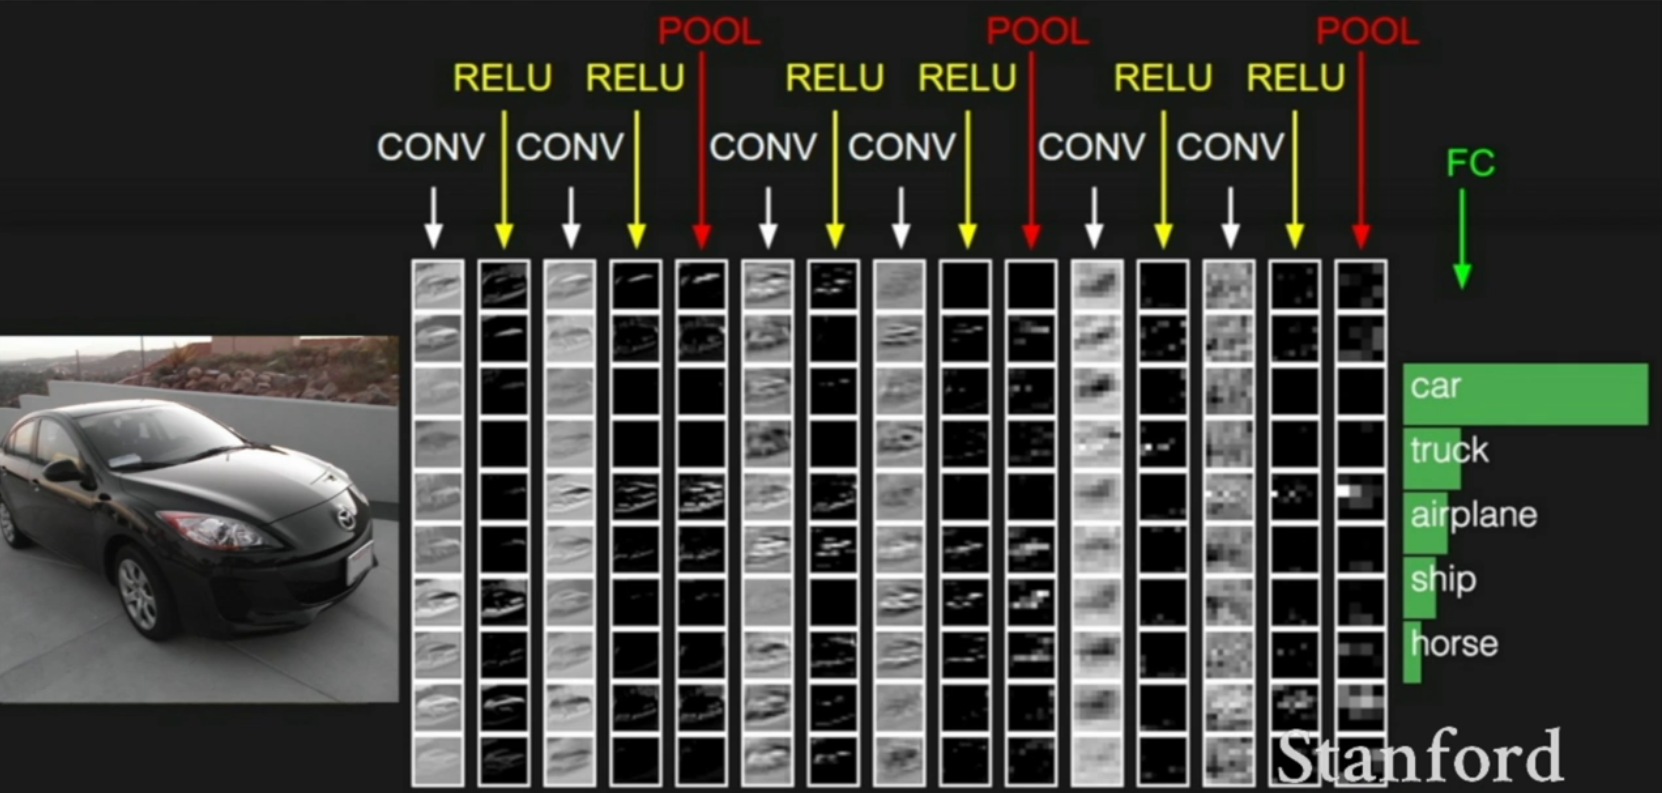
\includegraphics[width=\linewidth]{Pics/cexample.png}
	\caption{Fully Connected Layer}
\end{figure}

\end{frame}

\begin{frame}
\frametitle{Pooling}

\begin{figure}
	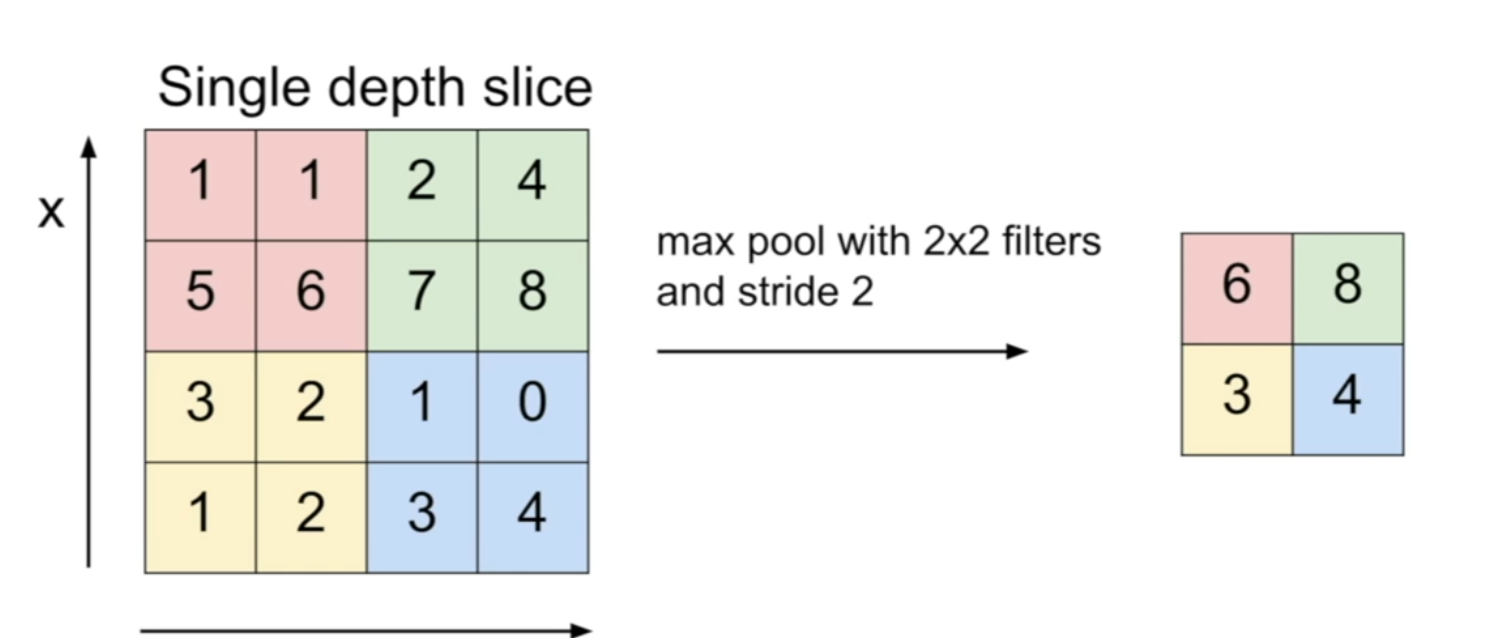
\includegraphics[width=\linewidth]{Pics/pooling.png}
	\caption{Max-pooling}
\end{figure}

\end{frame}

\begin{frame}
\frametitle{CNN}

\begin{figure}
	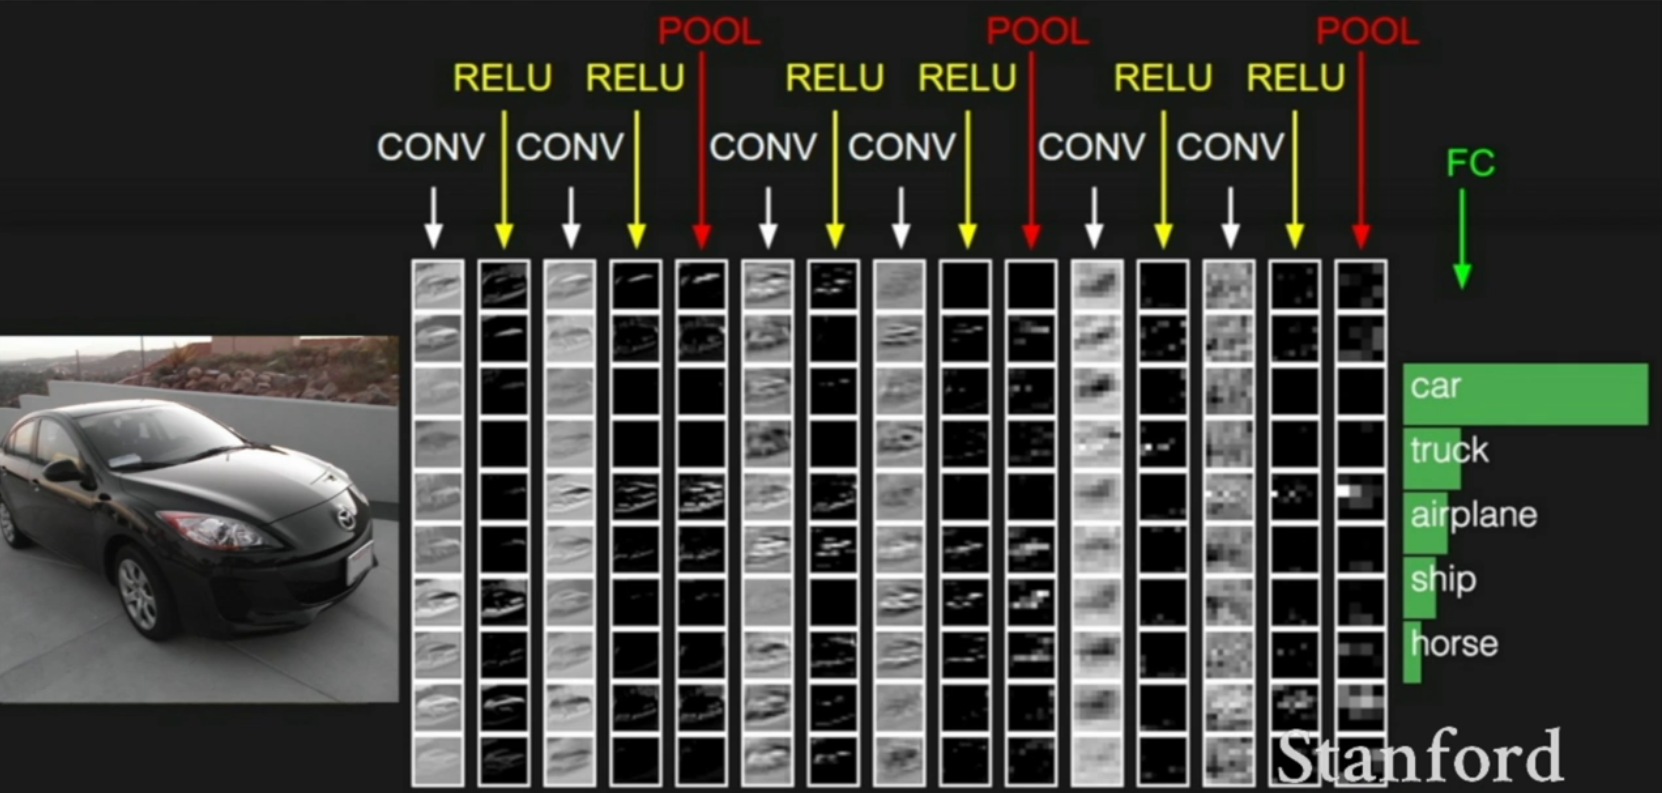
\includegraphics[width=\linewidth]{Pics/cexample.png}
	\caption{Fully Connected Layer}
\end{figure}

\end{frame}



\begin{frame}
\frametitle{Comparing}

\begin{figure}
	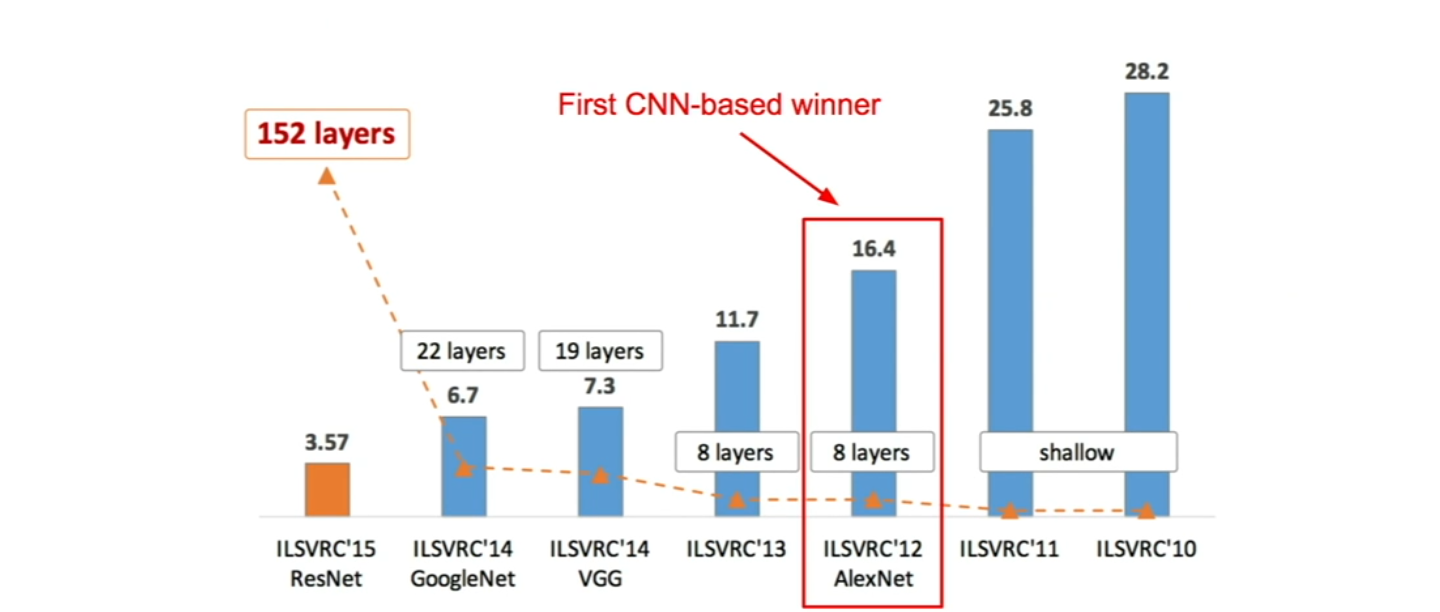
\includegraphics[width=\linewidth]{Pics/comaprecnn.png}
	\caption{Comparing Structures}
\end{figure}

\end{frame}

\begin{frame}
\frametitle{AlexNet}

\begin{figure}
	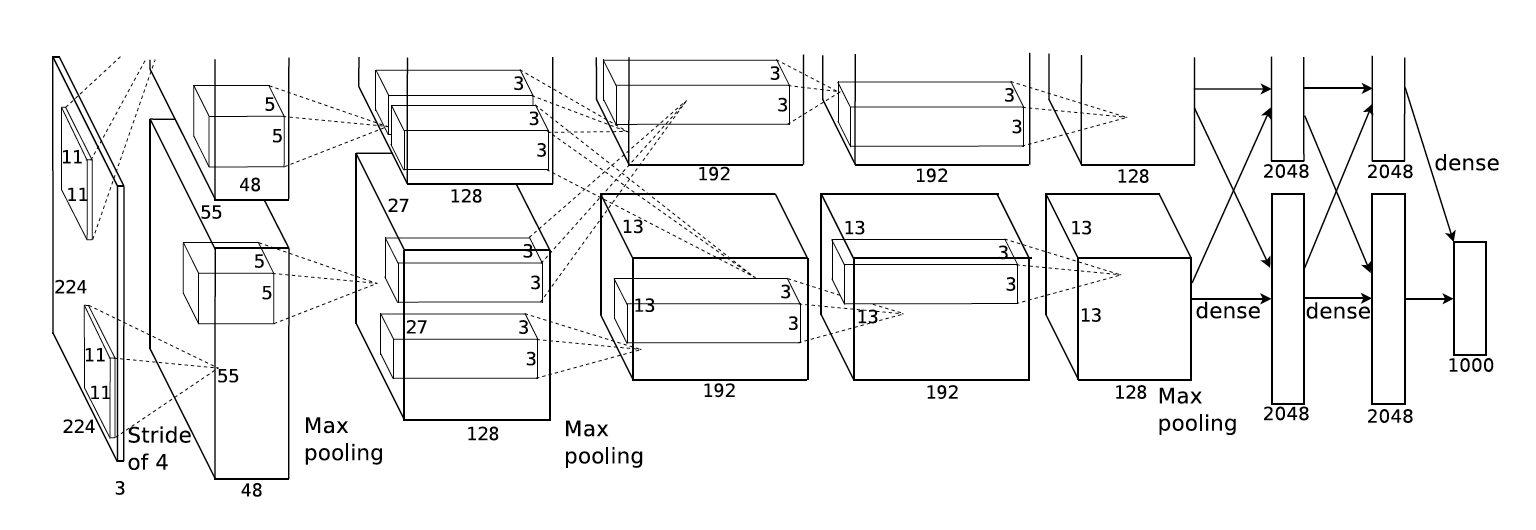
\includegraphics[width=\linewidth]{Pics/alexnet.png}
	\caption{AlexNet architecture}
\end{figure}

\end{frame}

\begin{frame}
\frametitle{AlexNet}

\begin{figure}
	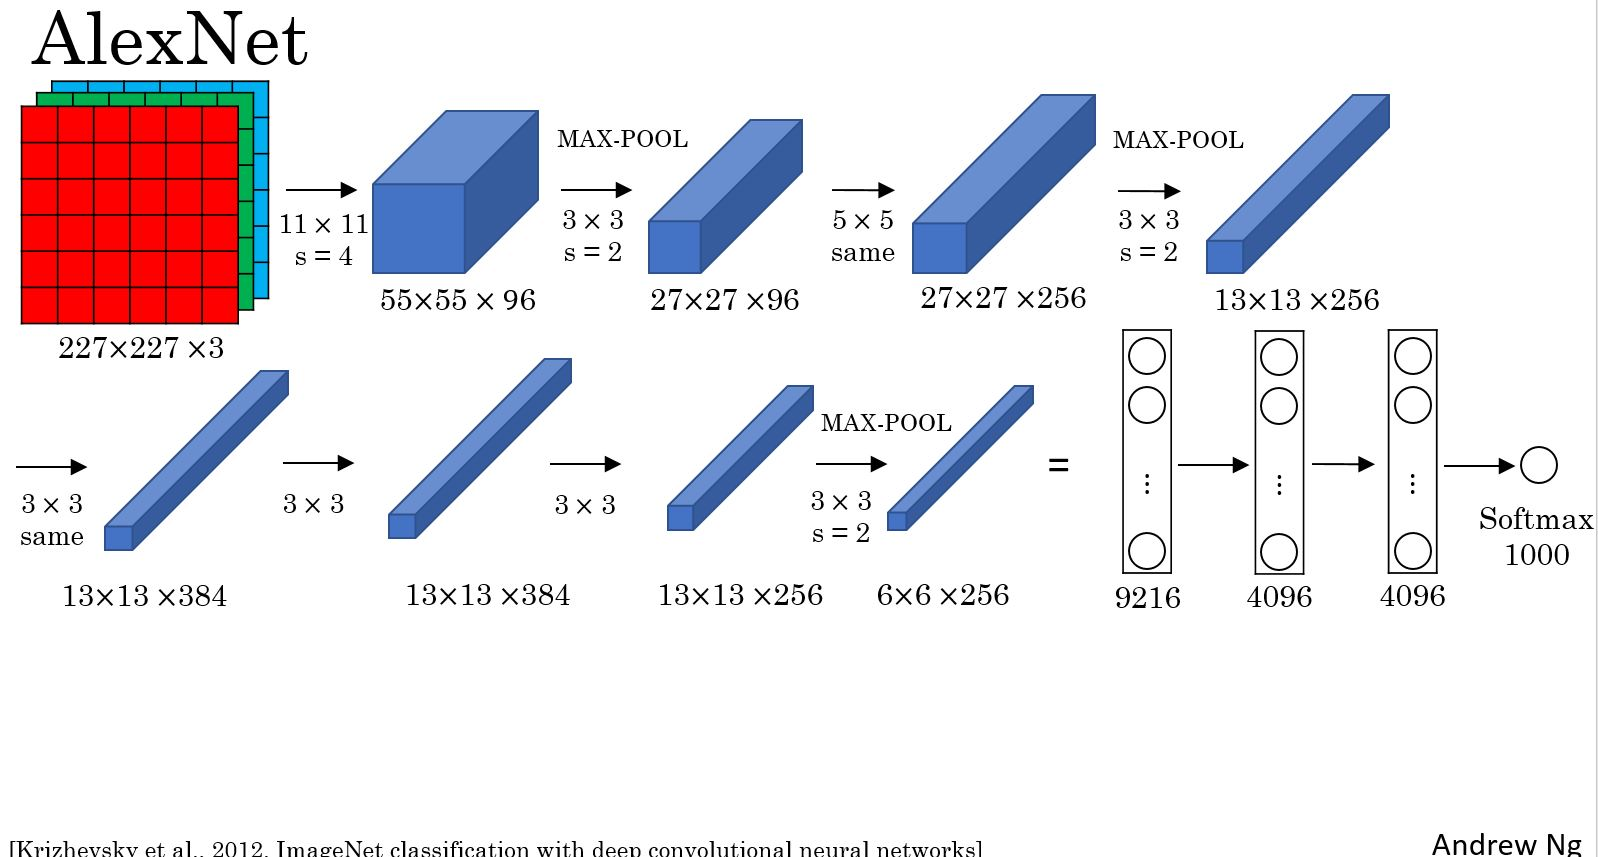
\includegraphics[width=\linewidth]{Pics/alexnetarch.jpg}
	\caption{AlexNet architecture}
\end{figure}

\end{frame}

\begin{frame}
\frametitle{Comparing}

\begin{figure}
	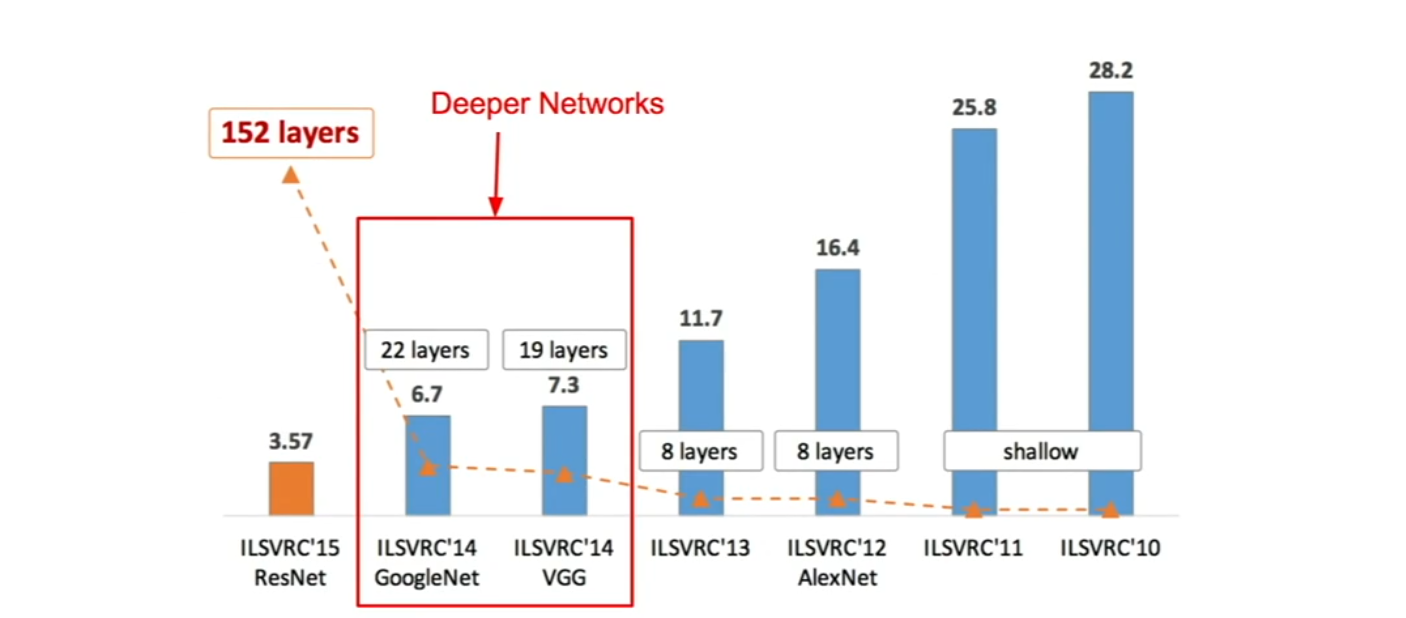
\includegraphics[width=\linewidth]{Pics/compare2.png}
	\caption{Comparing Structures}
\end{figure}

\end{frame}


\begin{frame}
\frametitle{VGG}
{\color{red} Deeper Networks, Smaller Filters}
\begin{figure}
	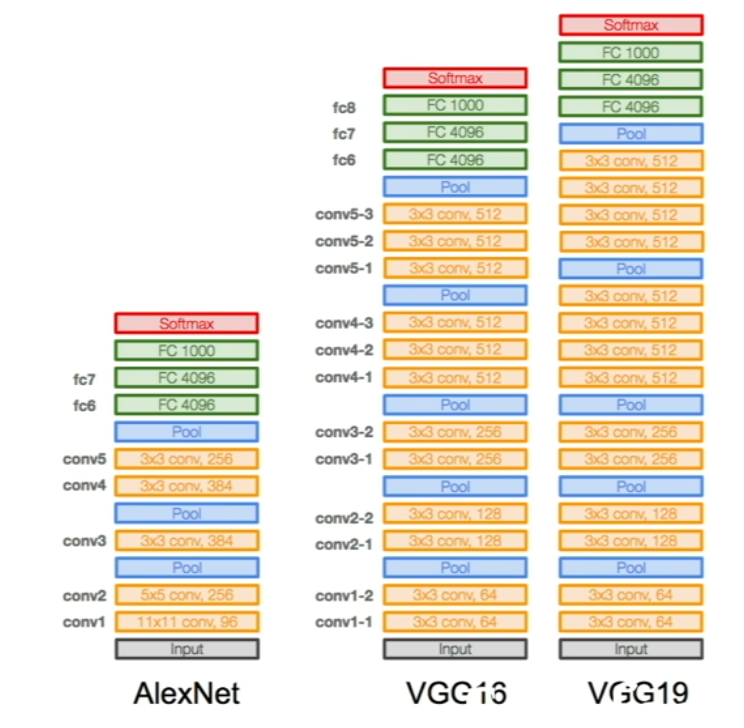
\includegraphics[width=.6\linewidth]{Pics/VGG.png}
	\caption{VGG Structures}
\end{figure}

\end{frame}
\begin{frame}
\frametitle{Comparing}

\begin{figure}
	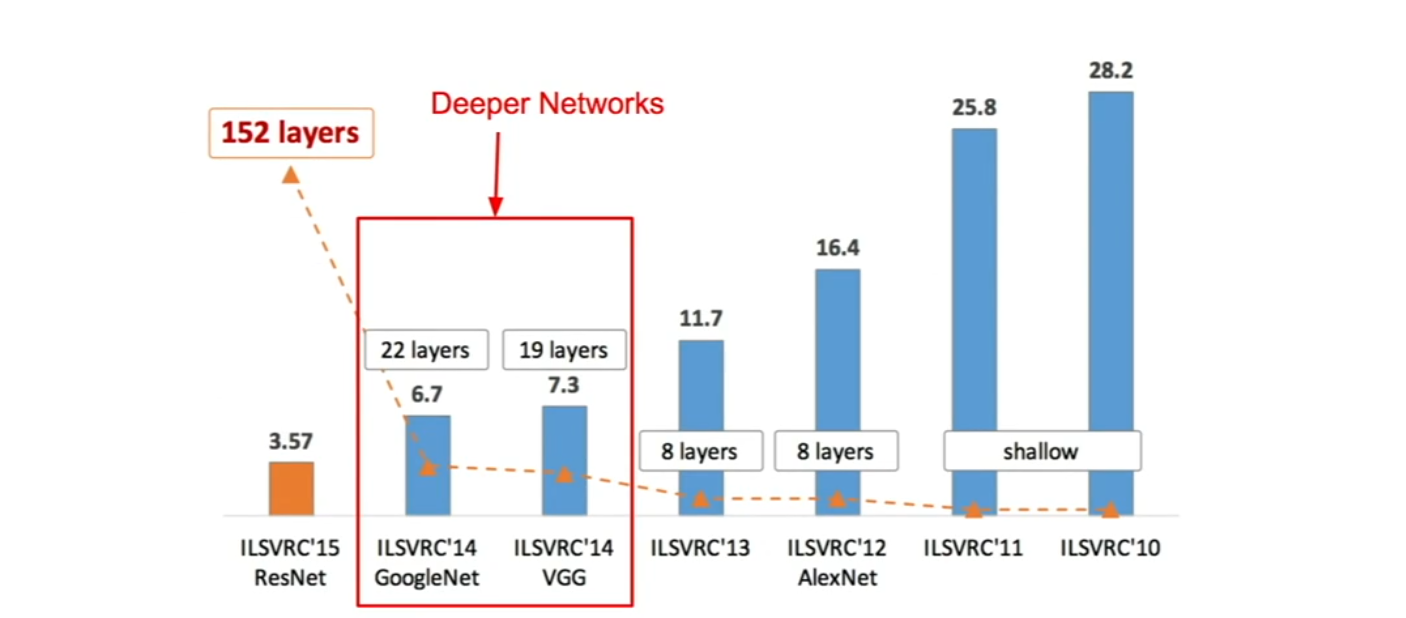
\includegraphics[width=\linewidth]{Pics/compare2.png}
	\caption{Comparing Structures}
\end{figure}

\end{frame}

\begin{frame}[fragile]
\frametitle{GoogLeNet}
{\color{red} Make deeper networks computationally inexpensive}
\begin{figure}
	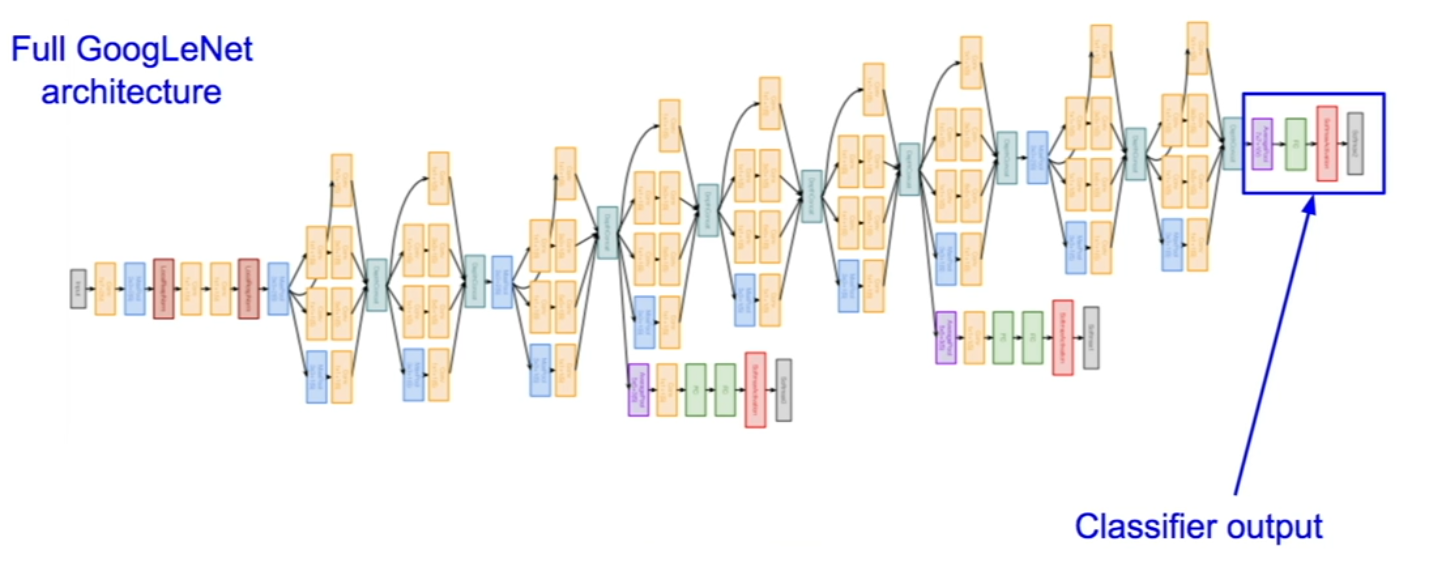
\includegraphics[height=0.3\textheight]{Pics/googlenet.png}
\end{figure}
\begin{figure}
	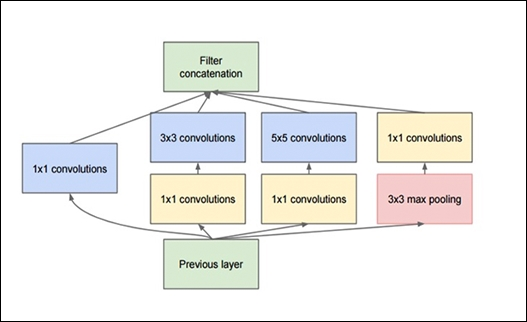
\includegraphics[height=0.4\textheight]{Pics/inception.jpg}
\end{figure}
\end{frame}

\begin{frame}
\frametitle{Comparing}

\begin{figure}
	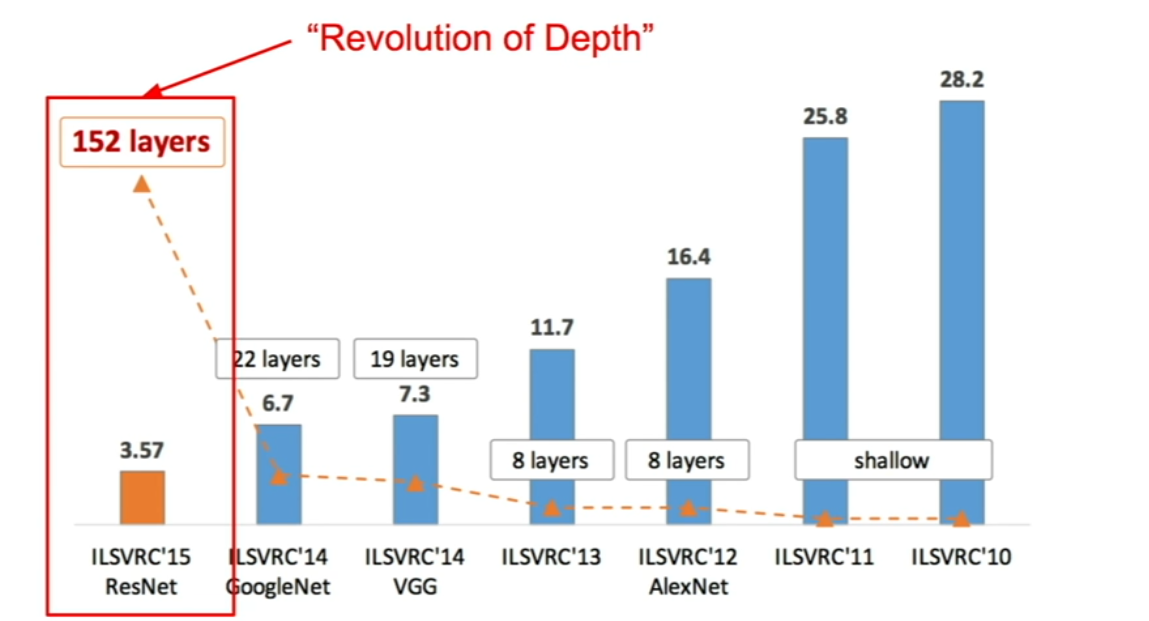
\includegraphics[width=\linewidth]{Pics/com3.png}
	\caption{Comparing Structures}
\end{figure}

\end{frame}

\begin{frame}
\frametitle{ResNet}

\begin{figure}
	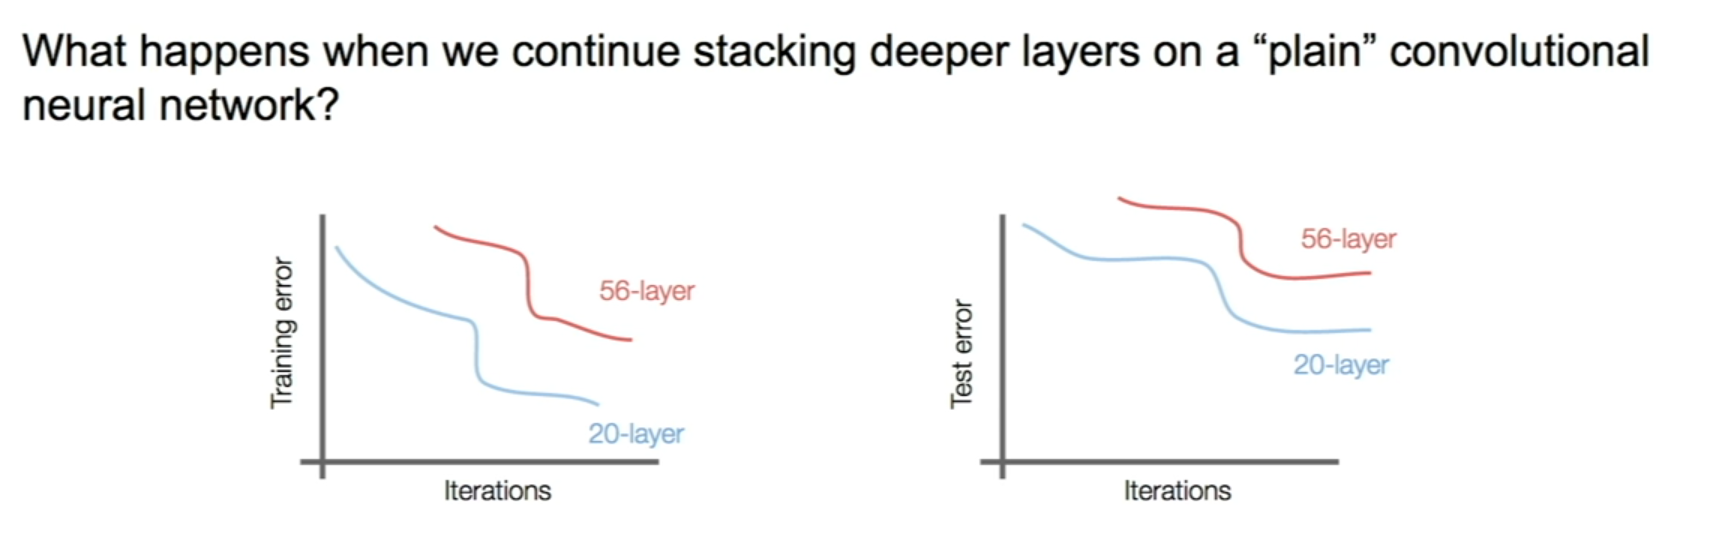
\includegraphics[width=\linewidth]{Pics/plain.png}
\end{figure}

\end{frame}

\begin{frame}
\frametitle{ResNet}

\begin{figure}
	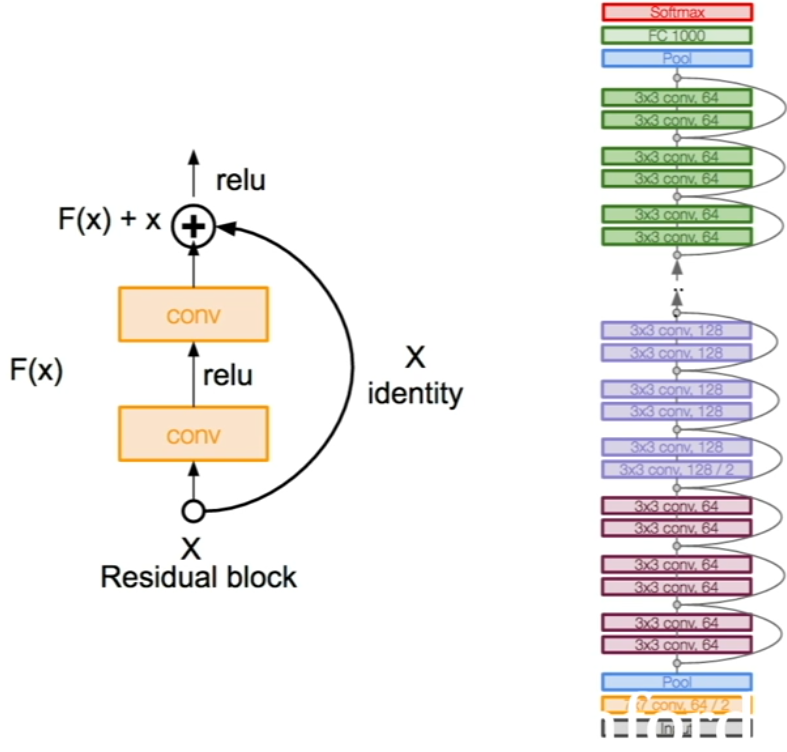
\includegraphics[width=.6\linewidth]{Pics/resnet.png}
	\caption{ResNet Architecture}
\end{figure}

\end{frame}
\begin{frame}
	
\frametitle{Comparing}

\begin{figure}
	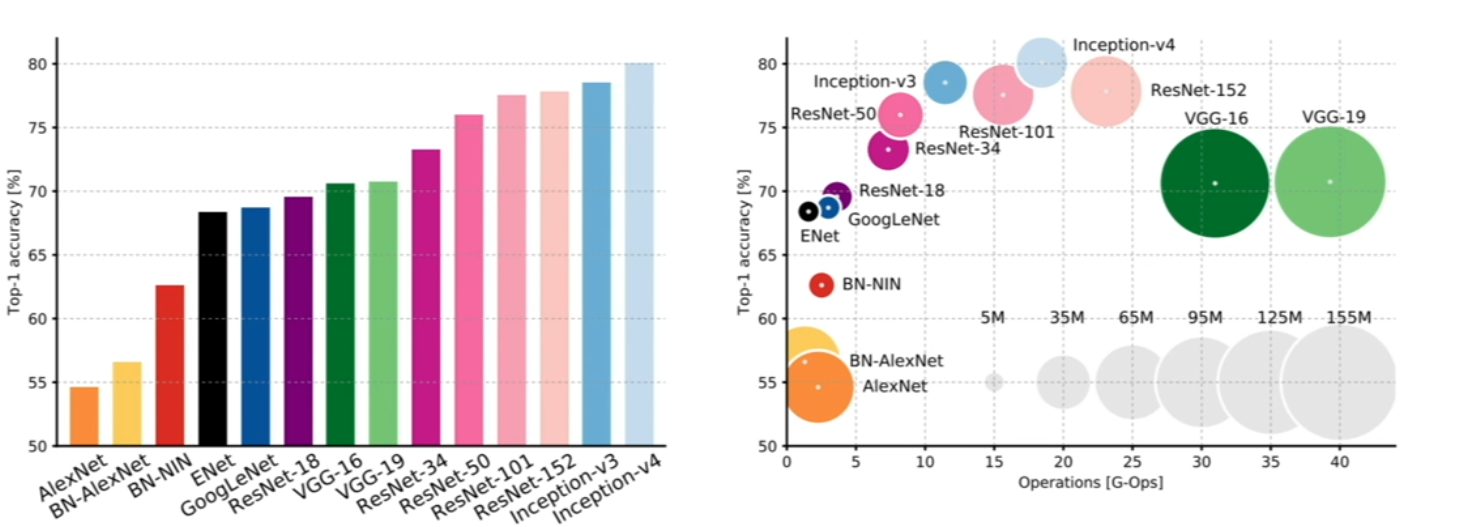
\includegraphics[width=\linewidth]{Pics/ccomplex.png}
	\caption{Comparison}
\end{figure}

\end{frame}


\begin{frame}
\frametitle{Example}
\begin{figure}

	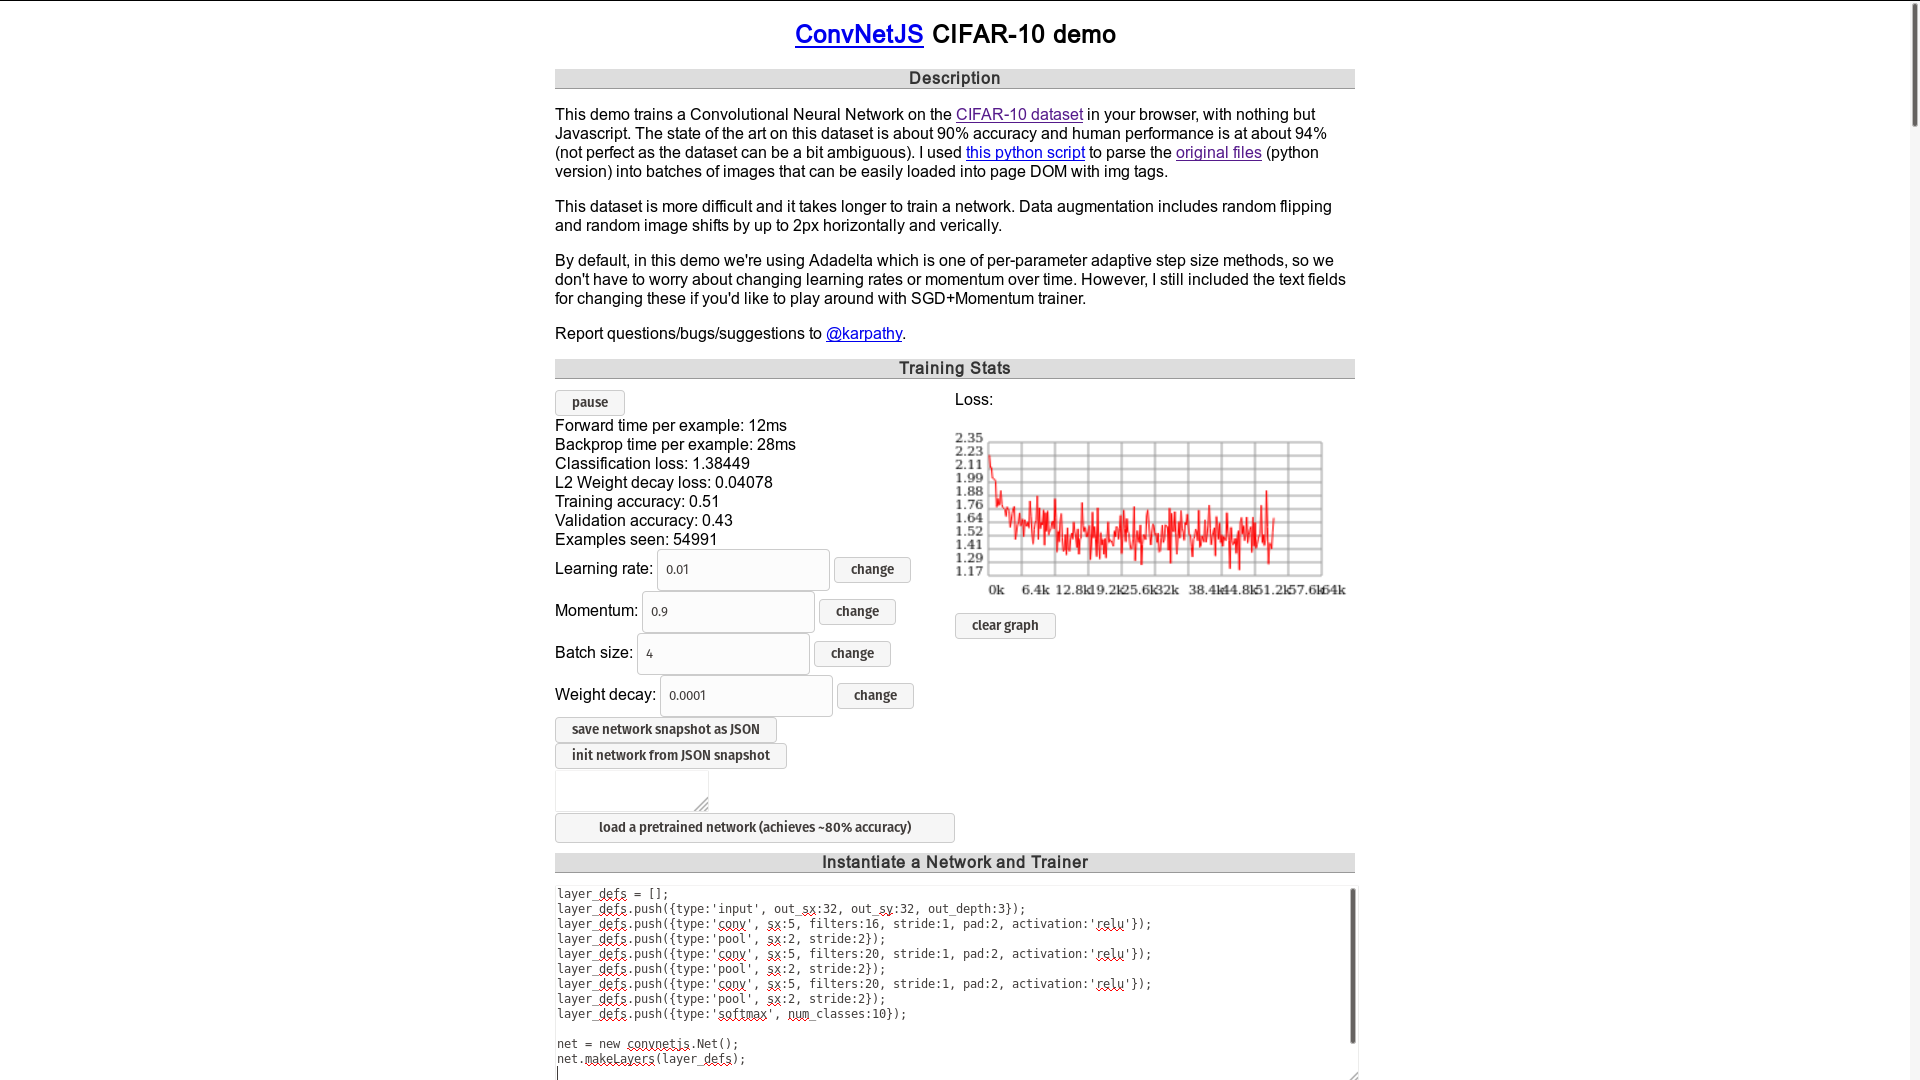
\includegraphics[width=\linewidth]{Pics/cnnex.png}
\end{figure}

\end{frame}
	
	
	
\section{Localization}
\begin{frame}
	\frametitle{Computer Vision Tasks}
	
	\begin{figure}
		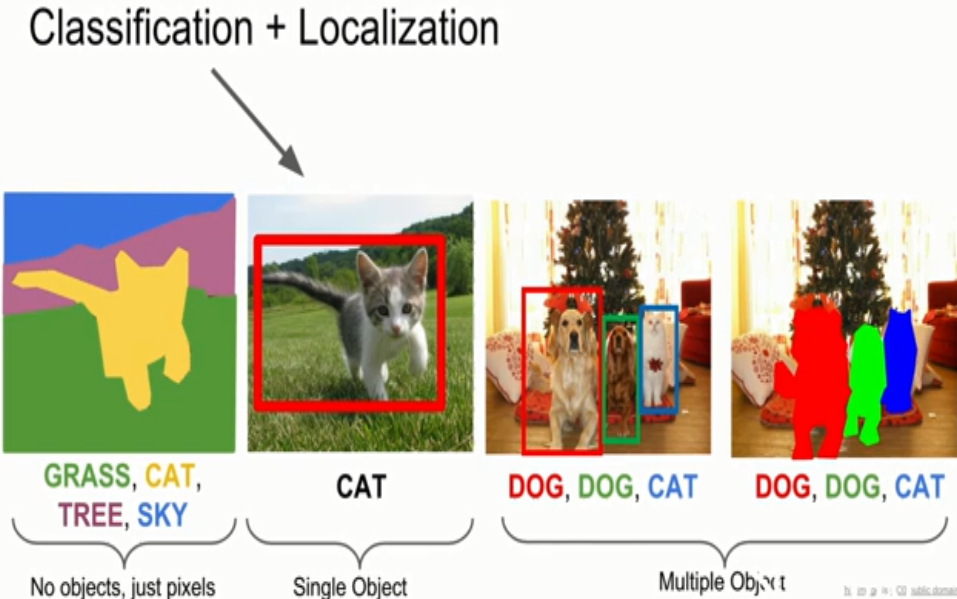
\includegraphics[width=\linewidth]{Pics/classloc.PNG}
		
	\end{figure}
	
\end{frame}
\begin{frame}
	\frametitle{Classification + Localization}
	\begin{figure}
		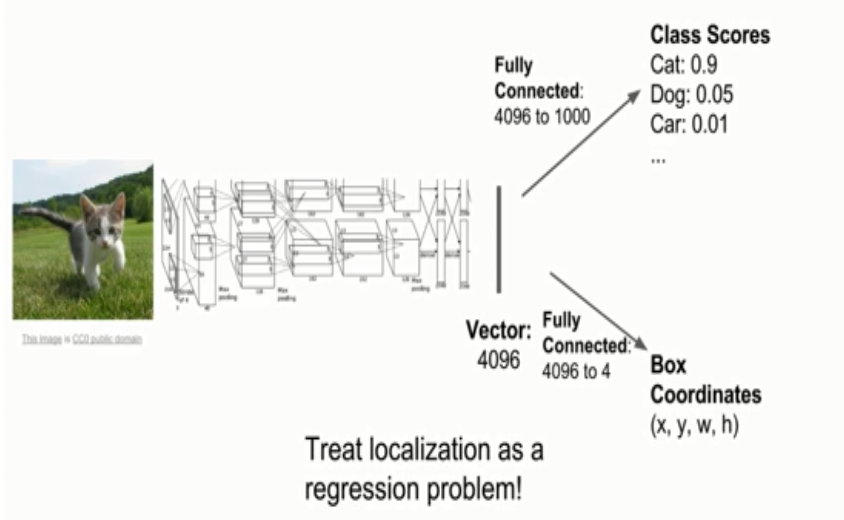
\includegraphics[width=\linewidth]{Pics/loc2.PNG}
	\end{figure}
	
\end{frame}
\begin{frame}
	\frametitle{Example}
	
	\begin{figure}
		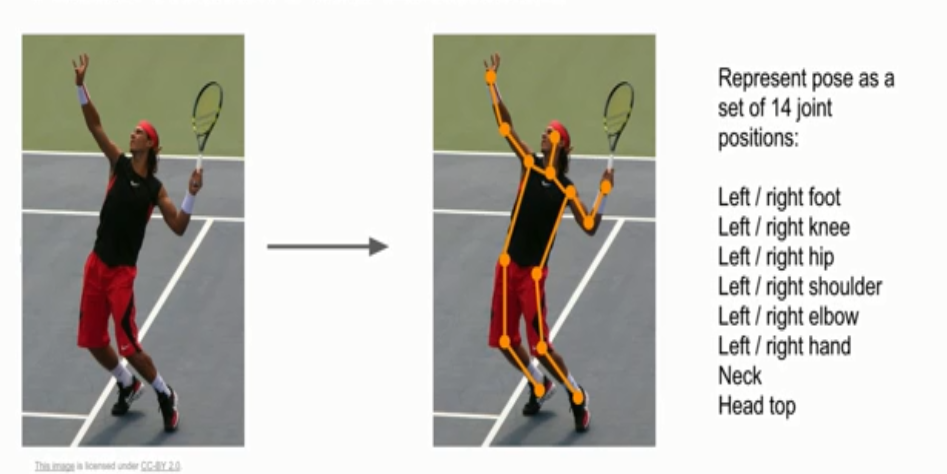
\includegraphics[width=\linewidth]{Pics/humanpose.PNG}
		\caption{Body pose estimation}
	\end{figure}
	
\section{Object Detection}
\end{frame}
\begin{frame}
	\frametitle{Fancier Task}
	
	\begin{figure}
		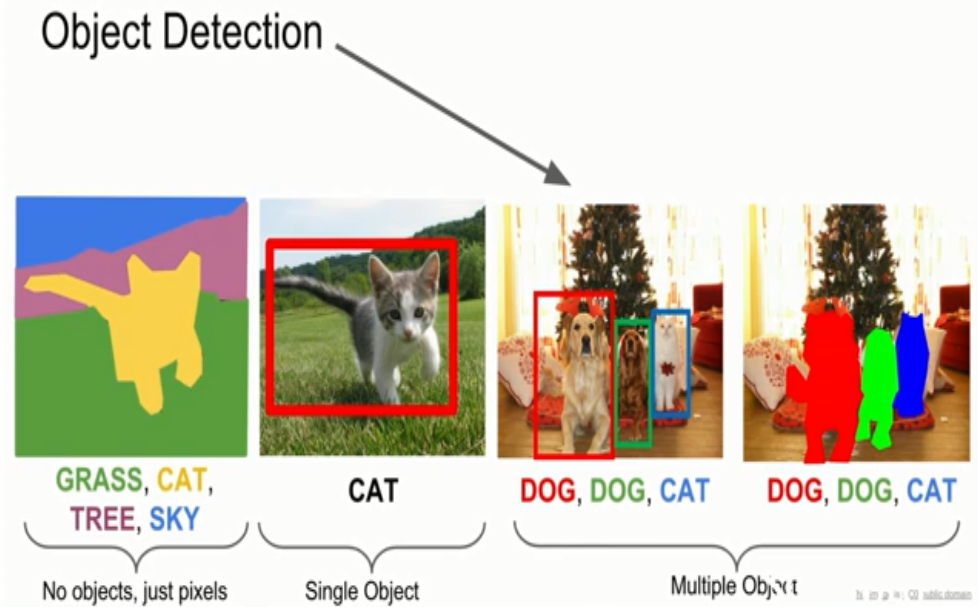
\includegraphics[width=\linewidth]{Pics/detect1.PNG}
		
	\end{figure}
	
\end{frame}
\begin{frame}
	\frametitle{Object Detection}
	\begin{figure}
		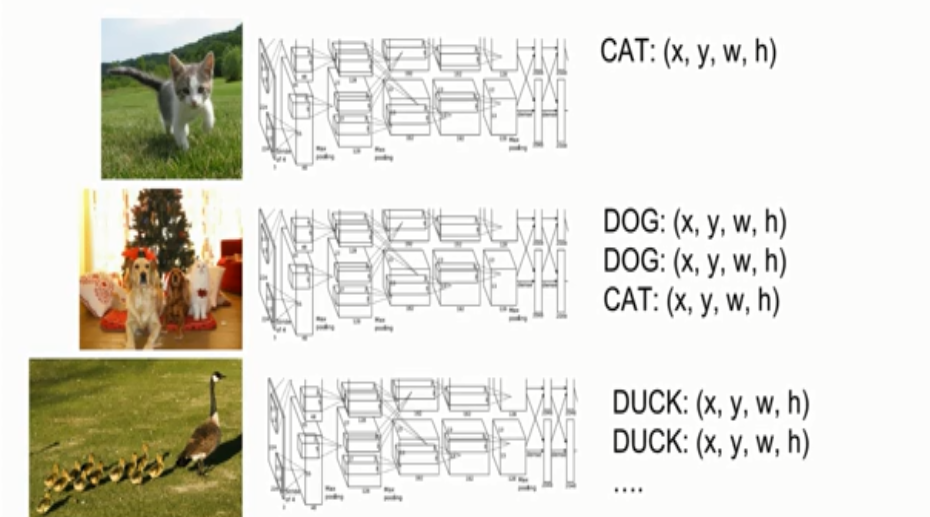
\includegraphics[width=\linewidth]{Pics/objectdetect.PNG}
		\caption{{\color{red}New approach is needed}}
	\end{figure}
	
\end{frame}
\begin{frame}
	\frametitle{Object Detection}
	
	\begin{figure}
		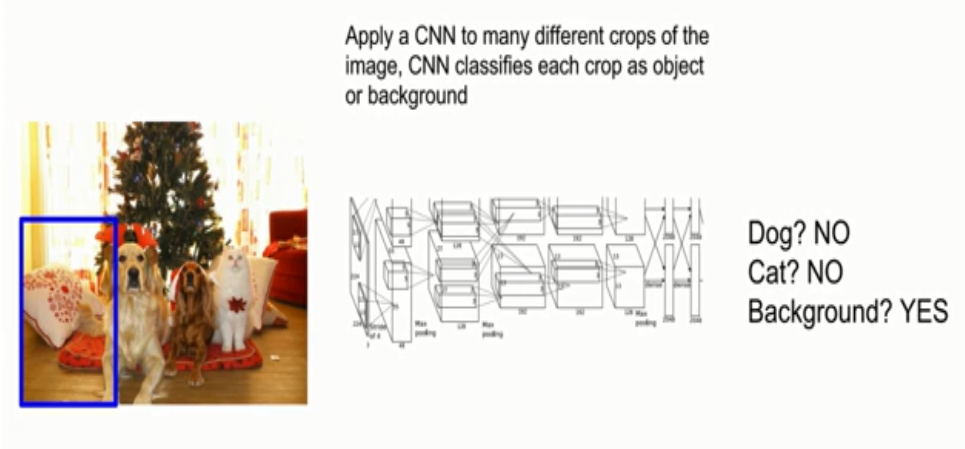
\includegraphics[width=\linewidth]{Pics/objectdetect2.PNG}
		
	\end{figure}
	
\end{frame}
\begin{frame}
	\frametitle{RCNN}
	
	\begin{figure}
		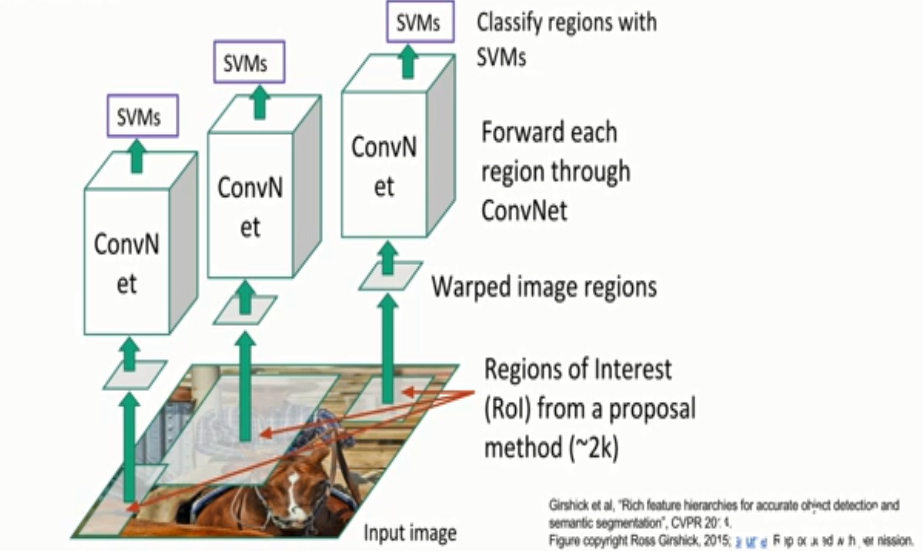
\includegraphics[width=\linewidth]{Pics/rcnn.PNG}
		
	\end{figure}
	
\end{frame}
\begin{frame}
	\frametitle{Fast RCNN}
	
	\begin{figure}
		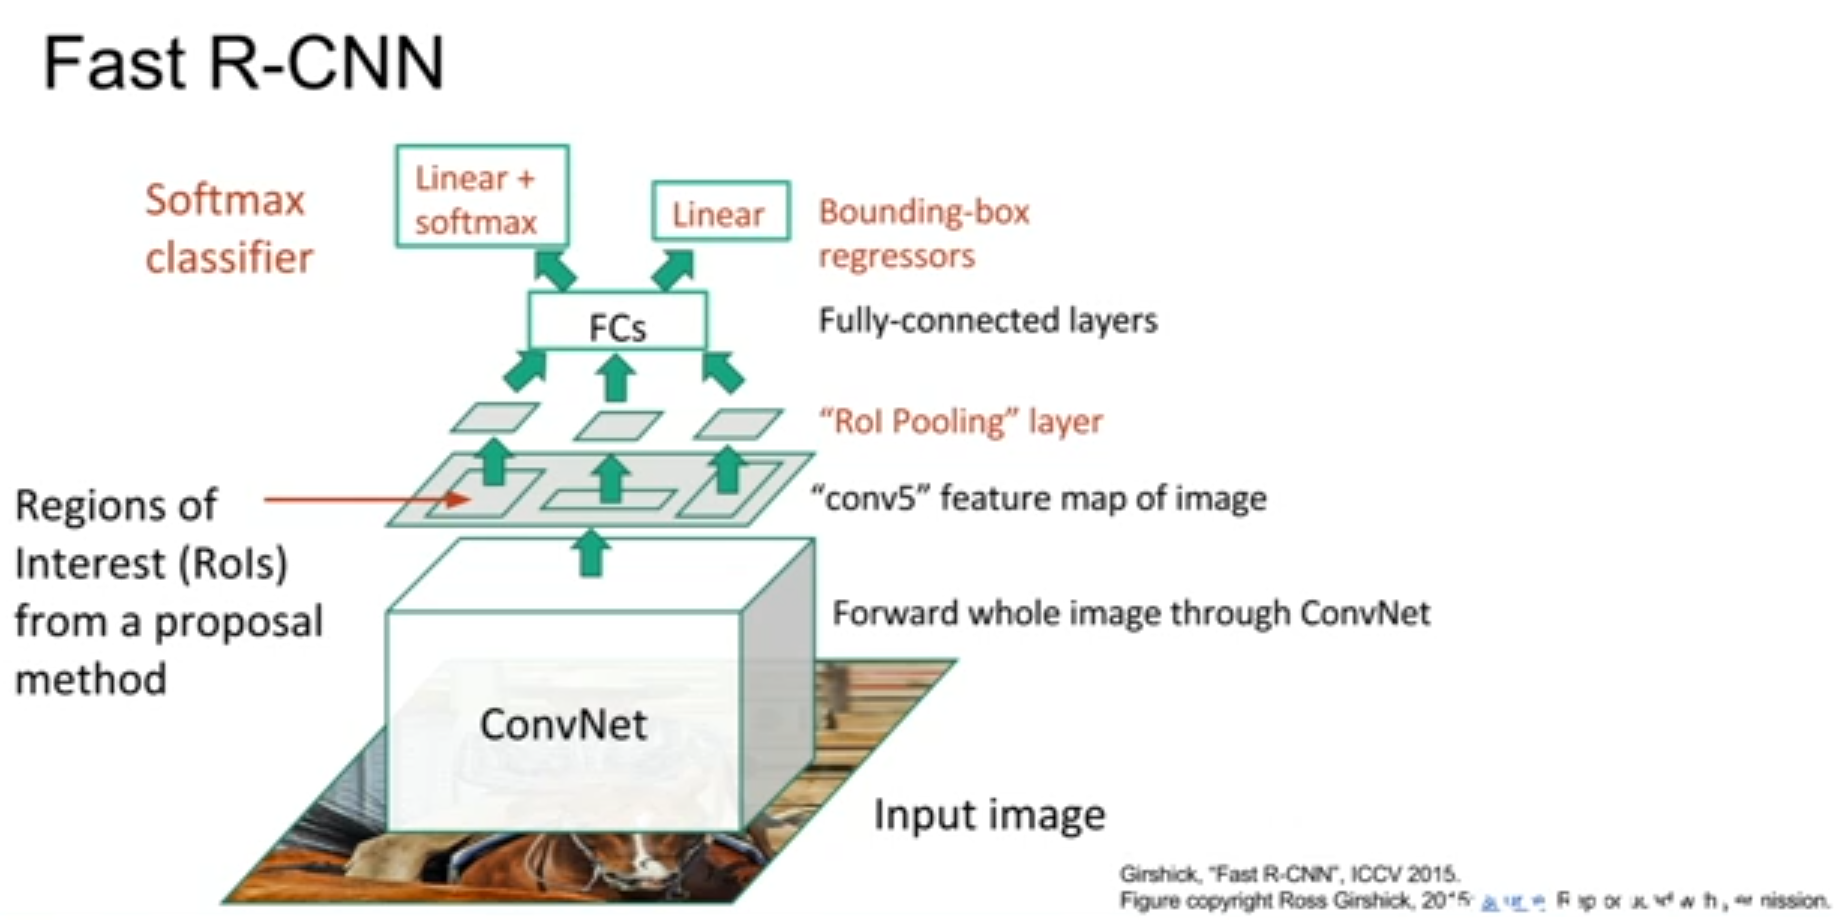
\includegraphics[width=\linewidth]{Pics/fastrcnn.PNG}
		
	\end{figure}
	
\end{frame}
\begin{frame}
	\frametitle{Comparing}
	
	\begin{figure}
		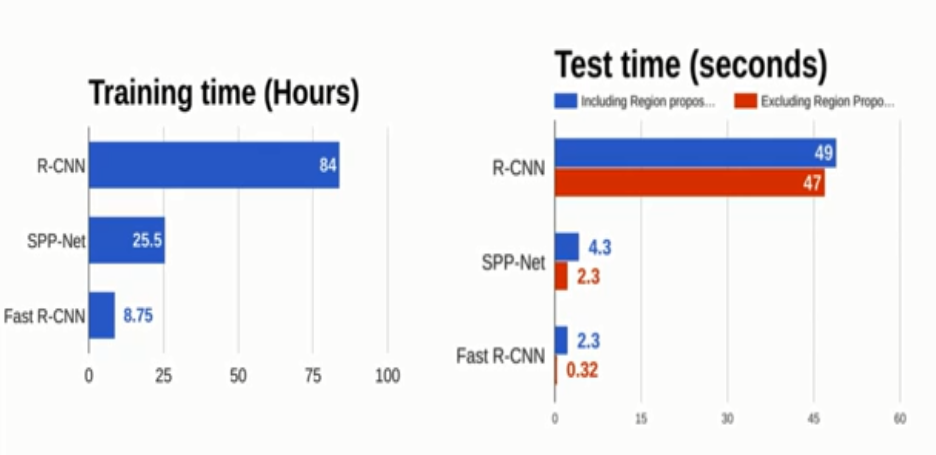
\includegraphics[width=\linewidth]{Pics/crcnn.PNG}
		
	\end{figure}
	
\end{frame}
\begin{frame}
\frametitle{Even Faster}
\begin{figure}
	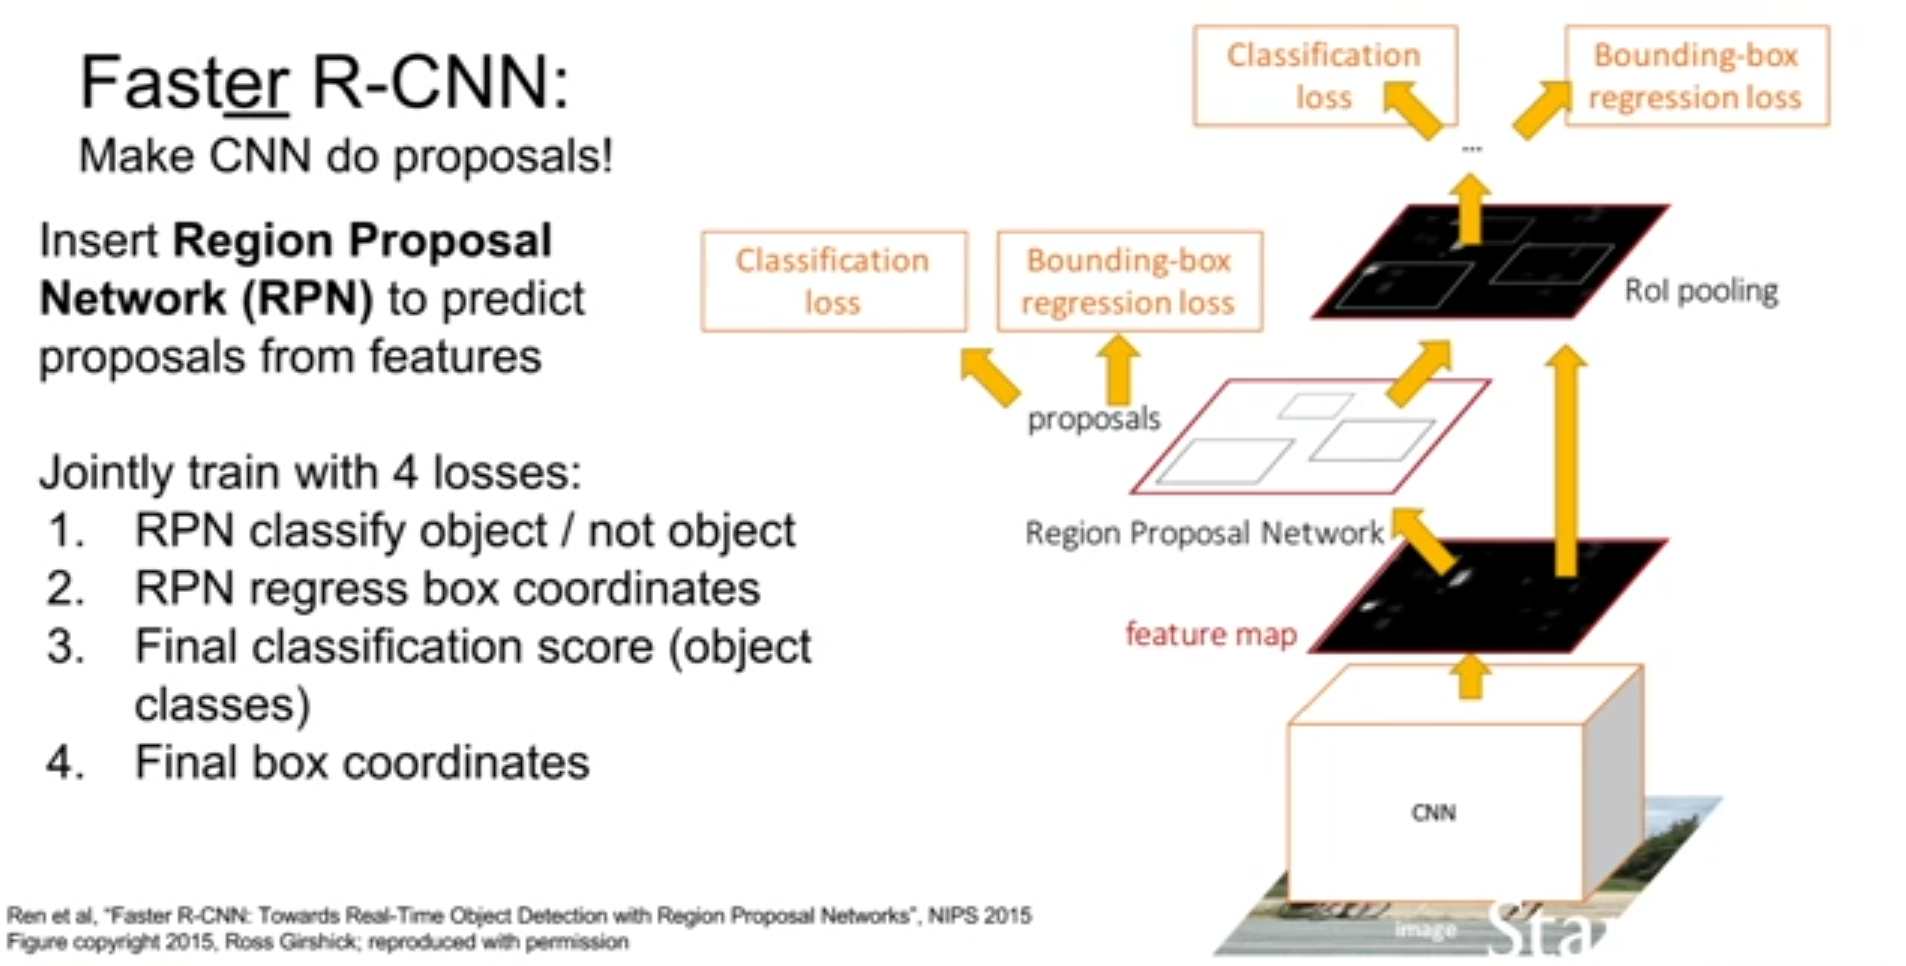
\includegraphics[width=\linewidth]{Pics/FasterRCNN.png}
\end{figure}
\end{frame}

\begin{frame}
\frametitle{Even Faster}

\begin{figure}
	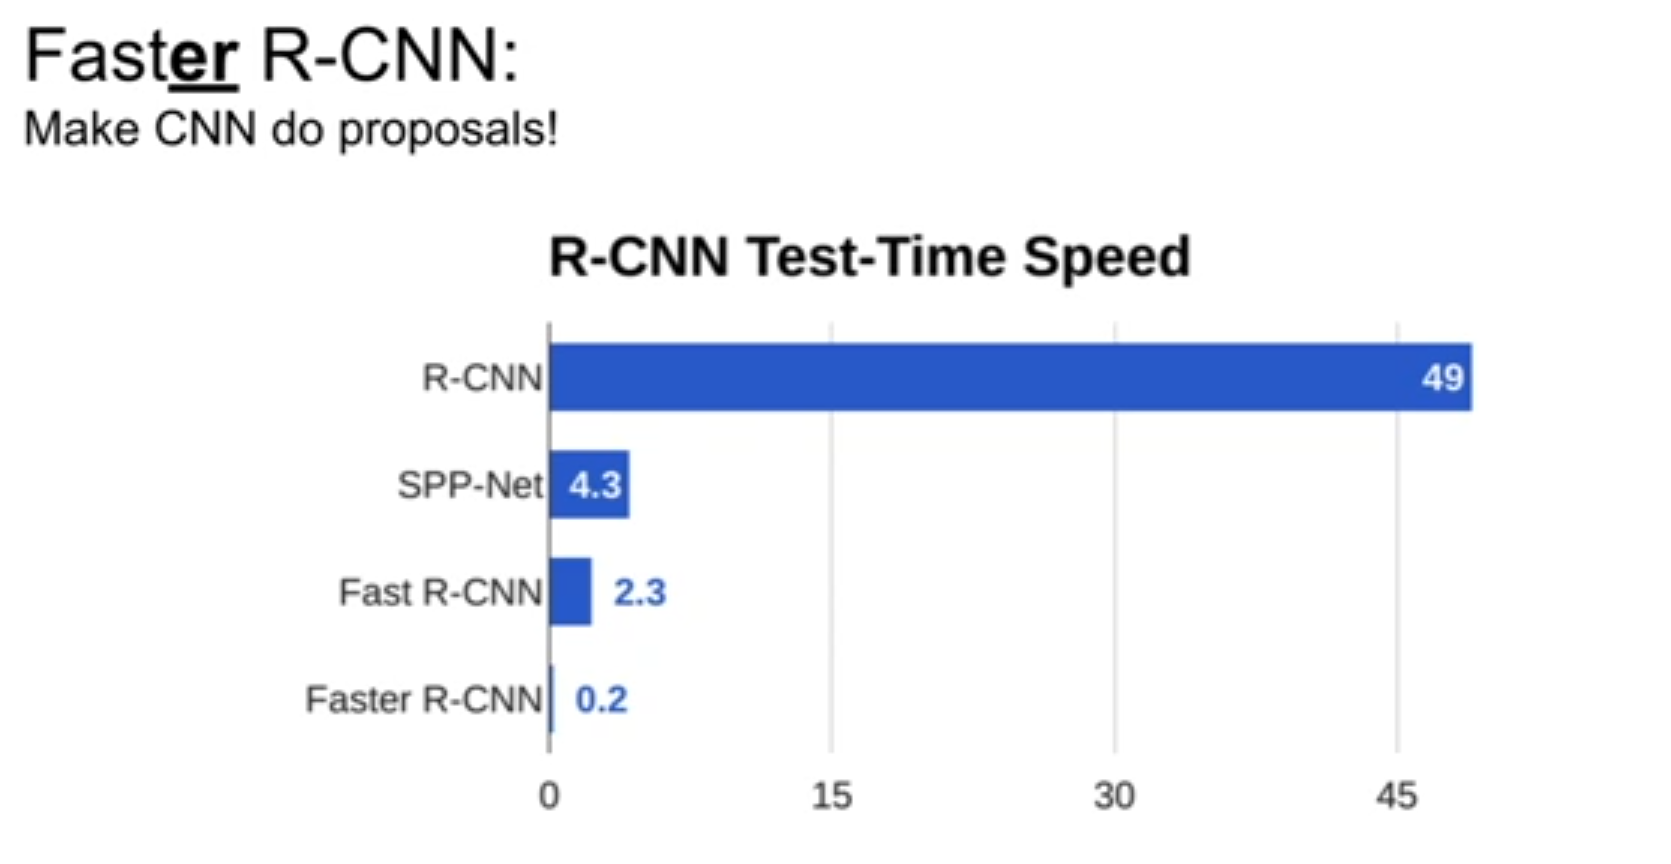
\includegraphics[width=\linewidth]{Pics/fastercompare.png}
	
\end{figure}

\end{frame}

\begin{frame}
	\frametitle{Yolo}
	\begin{figure}
		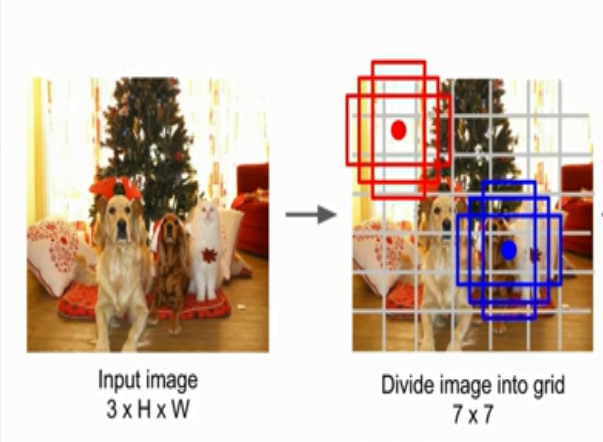
\includegraphics[width= .8\linewidth]{Pics/yolo.PNG}
	\end{figure}
\end{frame}

\begin{frame}
\frametitle{References}
	References:
	\begin{itemize}
		\item
		Krizhevsky, Alex \& Sutskever, Ilya \& E. Hinton, Geoffrey. (2012). ImageNet Classification with Deep Convolutional Neural Networks. Neural Information Processing Systems. 25. 10.1145/3065386.
		\item
		Very Deep Convolutional Networks for Large-Scale Image Recognition
		Karen Simonyan, Andrew Zisserman
		(Submitted on 4 Sep 2014 (v1), last revised 10 Apr 2015 (this version, v6))
		\item
		Going Deeper with Convolutions
		Christian Szegedy, Wei Liu, Yangqing Jia, Pierre Sermanet, Scott Reed, Dragomir Anguelov, Dumitru Erhan, Vincent Vanhoucke, Andrew Rabinovich
		(Submitted on 17 Sep 2014)
		\item Stanford CS231n 2017
	\end{itemize}
\end{frame}

\begin{frame}
\Huge
\centering
Any Question?
\end{frame}

\end{document} 